\section{Esempi di categorie nella pratica matematica}\label{sec_esempi_cats}
Iniziamo ora a dare degli esempi di categorie piccole partendo dall'esempio più semplice, anche quello più banale.
\subsection{Categorie come forme}\label{ssec:categorie_forme}
\begin{example}\label{ex_cat_vuota}\index{Categoria!--- vuota}
	La \emph{categoria vuota} o \emph{categoria iniziale} \(\ctInit\) non ha oggetti né morfismi. Più formalmente, \(\ctC_0,\ctC_1\) sono le classi vuote, e non è necessario specificare altra struttura per soddisfare (vacuamente) tutti gli assiomi di categoria.
\end{example}
\begin{example}\label{ex_cat_term}\index{Categoria!--- terminale}
	La \emph{categoria terminale} \(\ctTerm\) ha un solo oggetto \(\bullet\), e un unico morfismo \(\id_\bullet : \bullet\to\bullet\) che fa da identità. Chiaramente, non si può fare altro che porre \(\id_\bullet\cmp\id_\bullet=\id_\bullet\), e tutti gli assiomi di categoria sono soddisfatti.
\end{example}
\index{Categoria!--- discreta}
\`E sempre possibile dotare un insieme \(A\) della topologia discreta (o `massimale'), dove ogni sottoinsieme \(U\) di \(A\) è aperto, e della topologia indiscreta (o `minimale'), dove solo \(\varnothing\) e \(A\) sono aperti. Similmente, esistono due maniere, massimale e minimale, di considerare un insieme\footnote{Riguardo al problema se sia possibile dotare una classe propria della struttura di categoria discreta, la questione \emph{sembra} banale, ma in realtà tutt'altro che semplice da discutere: sebbene non ci sia alcun apparente problema ad assumere l'esistenza di classi proprie discrete, queste spesso vengono proibite \emph{ab imis} assumendo un assioma a parte in aggiunta ai soliti della teoria degli insiemi/classi, detto \emph{principio di Vop\v enka}: questo assioma afferma, precisamente, che non esistono sottoclassi proprie discrete nella classe propria di tutti gli insiemi.} \(A\) una categoria.
\paolo{c'è del materiale introduttivo sul principio di Vopenka a cui possiamo rimandare? (Il lettore potrebbe chiedersi che cosa significa "discreto" in teoria degli insiemi.)}
\begin{example}\label{ex_cat_discreta}\index{Categoria!--- discreta}
	Dato un insieme \(A\), la \emph{categoria discreta} su \(A\), denotata \(A^\delta\), ha per oggetti gli elementi \(a\in A\), un unico morfismo identità \(\id_a : a\to a\) per ogni \(a\), e nessun altro. La composizione è forzata a essere definita solamente tra identità, nel modo più ovvio possibile, e tutti gli assiomi di categoria sono ovviamente soddisfatti.
\end{example}
\begin{example}\label{ex_cat_codiscreta}\index{Categoria!--- codiscreta}
	Dato un insieme \(A\), la \emph{categoria codiscreta} su \(A\), denotata \(A^\chi\) ha per oggetti gli elementi \(a\in A\), per ogni coppia di oggetti \(a,a'\in A\) un unico morfismo \(u_{aa'}:a\to a'\), e la composizione è definita da \(u_{a'a''}\cmp u_{aa'}=u_{aa''}\) (in particolare, da questo segue che esiste un unico elemento \(\id_a=u_{aa}\in A^\chi(a,a)\)).
\end{example}
Alcune categorie che è spesso utile considerare si rappresentano mediante dei grafi:
\begin{example}\label{ex_cat_freccia}\index{Categoria!--- freccia generica}
	La categoria \(\genArrow\) detta \emph{freccia generica} ha due oggetti \(0,1\) e un unico morfismo non identità \(u : 0\to 1\) (che di solito non ha nome). La composizione è forzata a essere definita solamente tra le identità ed \(u\), nell'unico modo ovvio, e tutti gli assiomi di categoria sono banalmente soddisfatti.
\end{example}
\begin{example}\label{ex_cat_catena}\index{Categoria!--- catena generica}
	Più in generale, la categoria \(\Delta[n]\) detta \emph{catena generica di lunghezza \(n+1\)} è definita come segue:
	\begin{itemize}
		\item gli oggetti di \(\Delta[n]\) sono gli elementi di \(\{\iter[0]{n}\}\) (ci sono quindi \(n+1\) oggetti, per ogni \(n\ge 1\));\footnote{Si presti attenzione alla differente notazione per due insiemi finiti distinti: \(\bkt n := \{\iter n\}\), ma \([n] := \{\iter [0]n\}\) A volte è utile adottare la convenzione per cui quando \(n=-1\), l'insieme \(\{\iter[0]{n}\}\) è vuoto, e quindi la categoria `catena di lunghezza \(0\)' è la categoria vuota \(\ctInit\) di \ref{ex_cat_vuota}.}
		\item C'è un unico morfismo \(i\to j\) in \(\Delta[n]\) se e solo se \(i\le j\), di modo che esista un unico morfismo \(i\to i\) (l'identità) per ogni \(i\in\{\iter[0]{n}\}\), e un unico morfismo \(i\to i+1\) per \(i\in\{\iter[0]{n-1}\}\); in particolare l'unico morfismo \(i\to j\) è ottenuto dalla composizione
		      \[i\to i+1\to\dots\to j\]
	\end{itemize}
	\index{Simplesso}
	Le categorie \(\Delta[n]\) per \(=0,1,2,3\) sono rappresentate in figura \ref{fig:le_delta}.
	\begin{figure}[h]
		\begin{center}
			\begin{tikzpicture}[
					x=4em, y=4em,
					wrap/.style={fill=black!5, rounded corners},
					edge/.style={-latex},
					0simplex/.style={font=\scriptsize,inner sep=2pt},
				]
				\begin{scope}[xshift=0em,yshift=0.433*5em]
					\node[0simplex] (0D0) at (0.0,0) {0};
				\end{scope}
				\begin{scope}[xshift=4em,yshift=0.433*5em]
					\node[0simplex] (1D0) at (0.0,0) {0};
					\node[0simplex] (1D1) at (1.0,0) {1};
					\draw[edge] (1D0) -- (1D1);
				\end{scope}
				\begin{scope}[xshift=13em]
					\node[0simplex] (2D0) at (0.0,0) {0};
					\node[0simplex] (2D1) at (1.0,0) {1};
					\node[0simplex] (2D2) at (0.5,0.866) {2};
					\draw[edge] (2D0) -- (2D1);
					\draw[edge] (2D0) -- (2D2);
					\draw[edge] (2D1) -- (2D2);
				\end{scope}
				\begin{scope}[xshift=22em]
					\node[0simplex] (3D0) at (0.0,0) {0};
					\node[0simplex] (3D1) at (1.0,0) {1};
					\node[0simplex] (3D2) at (0.5,0.866) {2};
					\node[0simplex] (3D3) at (0.5,0.3) {3};
					\draw[edge] (3D0) -- (3D1);
					\draw[edge] (3D0) -- (3D2);
					\draw[edge] (3D1) -- (3D2);
					\draw[edge] (3D0) -- (3D3);
					\draw[edge] (3D1) -- (3D3);
					\draw[edge] (3D2) -- (3D3);
				\end{scope}
				\begin{scope}[on background layer]
					\path node[wrap, fit=(0D0)] (W0) {};
					\path node[wrap, fit=(1D0)(1D1)] (W1) {};
					\path node[wrap, fit=(2D0)(2D1)(2D2)] (W2) {};
					\path node[wrap, fit=(3D0)(3D1)(3D2)(3D3)] (W3) {};
					\node [below=2.5em of W0] (L) {$\Delta[0]$};
					\node at (L -| W1) {$\Delta[1]$};
					\node at (L -| W2) {$\Delta[2]$};
					\node at (L -| W3) {$\Delta[3]$};
				\end{scope}
			\end{tikzpicture}
		\end{center}
		\caption{Le categorie \(\Delta[0], \dots,\Delta[3]\). Si noti che non abbiamo rappresentato le frecce identità dei vari oggetti, e che la struttura di categoria che risulta è completamente determinata dalla struttura di grafo diretto. Ovviamente, \(\Delta[0]\) è la categoria terminale di \ref{ex_cat_term}, \(\Delta[1]\) è la freccia generica di \ref{ex_cat_freccia}. La categoria \(\Delta[n]\) spesso si chiama un \(n\)-\emph{simplesso}. }
		\label{fig:le_delta}
	\end{figure}
\end{example}
\paolo{non abbiamo ancora parlato di isomorfismi. Forse conviene rimandare il lettore a 2.4?}
\begin{example}\label{ex_cat_iso}\index{Categoria!--- isomorfismo generico}
	La categoria \emph{isomorfismo generico} \(\ctIso\) ha due oggetti ed esattamente una freccia fra ciascuna coppia di essi:
	\[\xymatrix@C=7ex{0 \ar@<.7ex>[r]^u \ar@(dl,ul)[] & 1 \ar@<.7ex>[l]^{u^{-1}} \ar@(ur,dr)[]}\]
	I due endomorfismi su \(0\) ed \(1\) devono quindi essere le identità, ed entrambe le composizioni dei morfismi non identità \(u\) e \(u^{-1}\) sono forzate ad essere l'identità sull'oggetto corrispondente. \`E quindi la categoria con due oggetti ed un unico isomorfismo fra di essi.
\end{example}
\begin{example}[Doppia freccia generica]\label{ex_cat_doppiafreccia}\index{Categoria!--- doppia freccia generica}
	La categoria \emph{doppia freccia generica} \(\{0\toto 1\}\) ha due oggetti \(0,1\) ed esattamente due morfismi non identità e paralleli \(s,t : 0\to 1\). La composizione è definita, ancora una volta, nell'unico modo ovvio, chiedendo che \(x\cmp \id_0=x=\id_1\cmp x\) per \(x\in\{s,t\}\).

	La doppia freccia è la `forma generica' di un grafo diretto (si veda \ref{ex_cat_libera}), dato che una coppia di funzioni \(s,t: E \toto V\) tra due insiemi consta precisamente di un digrafo che ha \(V\) per insieme dei vertici e \(E\) per insieme dei lati.
\end{example}
\begin{example}[Turcasso generico]\label{ex_cat_turcasso}\index{Turcasso}\index{Categoria!--- turcasso generico}
	Sia \(S\) un insieme; la categoria \(\turk\), detta \emph{turcasso generico} (con \(S\) elementi)\footnote{Il nome \emph{turcasso} denota un particolare tipo di faretra in uso agli arcieri turchi, solitamente fissata alla cintura dei soldati anziché portata a tracolla. Boccaccio scrive \cite{boccaccio1831teseide},
		\begin{verse}
			Dietro alle spalle un arco avea legato,\\
			Ed un turcasso di saette pieno,\\
			Che era d'oro tutto lavorato [\dots\unkern]
		\end{verse}} ha due oggetti \(0,1\), e una freccia \(s : 0\to 1\) per ogni \(s\in S\). La composizione è possibile solo tra \(s\in S\) e una identità, nel modo ovvio.

	Chiaramente se \(S=\varnothing\) si ottiene la categoria \(\{0,1\}^\delta\), discreta su \(\{0,1\}\); se \(\#S=2\) si ottiene la doppia freccia generica di \ref{ex_cat_doppiafreccia}.
\end{example}
\begin{example}\label{ex_quadcuboncubo}\index{Categoria!--- quadrato commutativo generico}
	La categoria \emph{quadrato commutativo generico} \(\ctQ\) ha 4 oggetti
	\[\{(00),(10),(01),(11)\} \]
	e una freccia \((ij)\to(kl)\) se e solo se \(i\le k\) e \(j\le l\); rappresentata graficamente, si tratta della categoria
	\[\begin{tikzcd}
			(00) \ar[r]\ar[d]\ar[dr]& (10)\ar[d] \\
			(01) \ar[r]& (11)
		\end{tikzcd}\]
	La composizione è forzata a essere definita cosicché la composizione \((00)\to (01)\to (11)\) sia uguale alla composizione \((00)\to (10)\to (11)\), e quindi la categoria \(\ctQ\) rappresenta la forma generica di un \emph{quadrato commutativo}.
\end{example}
\begin{remark}\index{Ordine prodotto}
	Si noti che \(\ctQ\) può essere pensato come un insieme ordinato, e precisamente l'insieme dei sottoinsiemi di un insieme con due elementi \(\{a,b\}\); in tal senso \((ij)\) rappresenta la funzione caratteristica \(\chi_U : \{a,b\}\to \{0,1\}\) di un sottoinsieme \(U\subseteq \{a,b\}\), nel senso che ad esempio \((10)=\{a\}, (00)=\varnothing\), eccetera. Si osservi anche che \(\ctQ\) è l'insieme parzialmente ordinato \(\genArrow\times \genArrow\), dotato dell'\emph{ordine prodotto} (si veda \ref{ord_sonocat} e \ref{cat_sonopos}).

	Quindi possiamo definire induttivamente
	\[P[0] = \Delta[0], \quad P[1] = \ctQ, \quad P[n+1] = P[n]\times \Delta[1]\]
	o (equivalentemente, nel senso che questa seconda definizione dà per ogni \(n\ge 0\) un \(P'[n]\) in biiezione con \(P[n]\), con una mappa che rispetta l'ordine) \(P'[n] = \pow {[n]} = \pow {\{0,1,\dots,n\}}\), cosicché l'insieme delle parti \(P[n]\) è il \emph{cubo commutativo \(n+1\)-dimensionale generico}: alcune \(P[n]\) per \(n=0,1,2,3\) sono raffigurate in \ref{fig_n_cubo}.
	\begin{figure}[h]
		\begin{center}
			\begin{tikzpicture}[x=8em, y=8em,
					wrap/.style={fill=black!5, rounded corners},
					edge/.style={-latex},
					subset/.style={font=\small\ttfamily},
				]
				\begin{scope}[xshift=0em,yshift=4em]
					\node[subset] (0D0) at (0.0,0) {0};
				\end{scope}
				\begin{scope}[xshift=2em,yshift=4em]
					\node[subset] (1D0) at (0.3,0) {0};
					\node[subset] (1D1) at (0.7,0) {1};
					\draw[edge] (1D0) -- (1D1);
				\end{scope}
				\begin{scope}[xshift=10em]
					\node[subset] (2D0) at (0.3,0.3) {00};
					\node[subset] (2D1) at (0.7,0.3) {01};
					\node[subset] (2D2) at (0.3,0.7) {10};
					\node[subset] (2D3) at (0.7,0.7) {11};
					\draw[edge] (2D0) -- (2D1);
					\draw[edge] (2D0) -- (2D2);
					\draw[edge] (2D2) -- (2D3);
					\draw[edge] (2D1) -- (2D3);
				\end{scope}
				\begin{scope}[xshift=22em]
					\node[subset] (3D0) at (0.3,0.3) {000};
					\node[subset] (3D1) at (0.7,0.3) {001};
					\node[subset] (3D2) at (0.3,0.7) {010};
					\node[subset] (3D3) at (0.7,0.7) {011};
					\node[subset] (3D4) at (0,0) {100};
					\node[subset] (3D5) at (1,0) {101};
					\node[subset] (3D6) at (0,1) {110};
					\node[subset] (3D7) at (1,1) {111};
					\draw[edge] (3D0) -- (3D1);
					\draw[edge] (3D0) -- (3D2);
					\draw[edge] (3D2) -- (3D3);
					\draw[edge] (3D1) -- (3D3);
					\draw[edge] (3D4) -- (3D5);
					\draw[edge] (3D4) -- (3D6);
					\draw[edge] (3D6) -- (3D7);
					\draw[edge] (3D5) -- (3D7);
					\draw[edge] (3D0) -- (3D4);
					\draw[edge] (3D1) -- (3D5);
					\draw[edge] (3D2) -- (3D6);
					\draw[edge] (3D3) -- (3D7);
				\end{scope}
				\begin{scope}[on background layer]
					\path node[wrap, fit=(0D0)] (W0) {};
					\path node[wrap, fit=(1D0)(1D1)] (W1) {};
					\path node[wrap, fit=(2D0)(2D1)(2D2)] (W2) {};
					\path node[wrap, fit=(3D4)(3D5)(3D6)(3D7)] (W3) {};
					\node [below=5em of W0] (L) {$P[0]$};
					\node at (L -| W1) {$P[1]$};
					\node at (L -| W2) {$P[2]$};
					\node at (L -| W3) {$P[3]$};
				\end{scope}
			\end{tikzpicture}
		\end{center}
		\caption{Le categorie \(P[n]\) per \(n=0,1,2,3\). La categoria \(P[n]\) si chiama un \(n\)-\emph{cubo}.}
		\label{fig_n_cubo}
	\end{figure}
\end{remark}
\begin{example}[Spanne e cospanne generiche]\label{ex_spancospan}\index{Categoria!--- spanna generica}
	\index{Categoria!--- cospanna generica|see {spanna generica}}
	La categoria \emph{spanna generica}
	\(\Lambda^2_0\) ha tre oggetti \(0,1,2\) e due morfismi non identità. Si raffigura come segue:\footnote{La scelta del termine si può intendere motivata dal fatto che una spanna è: la distanza (misurata dai codomini delle due frecce verso \(0,1\)) tra punta del pollice e punta del mignolo di una mano aperta adulta; l'arcata di un ponte (il cui punto più alto è l'oggetto \(0\)); le due braccia di un giogo (in inglese antico \emph{ġespan} era un giogo, un collare o per estensione un bracciale); un arcolaio (le cui braccia sono proprio \(1\leftarrow 0\to 2\); quest'ultima etimologia è dalla radice proto-indoeuropea \emph{*(s)penh\(_1\)-}, da cui derivano varie parole nel campo semantico di ciò che è capace di ruotare attorno a un asse).}
	\[\begin{tikzcd}
			1 & 0 \ar[r]\ar[l] & 2
		\end{tikzcd}\]
	La composizione è definita solamente quando almeno una delle due frecce è l'identità, ed è forzata da questo fatto.

	Dualmente, la categoria \emph{cospanna generica} \(\Lambda^2_2\) ha tre oggetti \(0,1,2\) ma i due morfismi non identità puntano verso \(2\) invece che uscire da \(0\):
	\[\begin{tikzcd}
			0\ar[r] & 2 & 1\ar[l]
		\end{tikzcd}\]
	Di nuovo, la composizione è definita solamente quando almeno una delle due frecce è l'identità.

	Si noti che \(\Lambda^2_2\) si ottiene da \(\Delta[2]\) `rimuovendo la freccia \(0\to 1\)', e analogamente \(\Lambda^2_0\) si ottiene rimuovendo la freccia \(1\to 2\).

	Più in generale, sia \(S\) un insieme; la categoria \emph{\(S\)-spanna generica} \(S^\lhd\) è definita come segue:
	\begin{itemize}
		\item gli oggetti di \(S^\lhd\) sono gli elementi di \(S^+ := S\cup \{-\infty\}\);
		\item esiste un unico morfismo \(f_s : -\infty\to s\), per ogni \(s\in S\).
	\end{itemize}
	La composizione è ancora una volta definita solamente quando almeno una delle due frecce è l'identità. Questo definisce una categoria in cui da un oggetto chiamato `\(-\infty\)' spiccano tante frecce \(f_s\) quanti sono gli elementi di \(S\).

	Dualmente, definiamo la categoria \emph{\(S\)-cospanna generica} \(S^\rhd\) come segue:
	\begin{itemize}
		\item gli oggetti di \(S^\rhd\) sono gli elementi di \(S^+ := S\cup \{+\infty\}\);
		\item esiste un unico morfismo \(f_s : s\to+\infty\), per ogni \(s\in S\).
	\end{itemize}
	La composizione è ancora una volta definita solamente quando almeno una delle due frecce è l'identità. Questo definisce una categoria in cui verso un oggetto chiamato `\(\infty\)' puntano tante frecce \(f_s\) quanti sono gli elementi di \(S\).

	Si noti che \(\Lambda^2_0=\{1,2\}^\lhd\) e \(\Lambda^2_2=\{0,1\}^\rhd\).
\end{example}
\begin{example}[Globo generico]\index{Categoria!--- globo generico}
	\label{ex_globo}
	La categoria \emph{globo generico} di dimensione \(n\ge 1\), denotata \(\ctGl(n)\), ha
	\begin{itemize}
		\item per oggetti i numeri naturali \(\iter[0]n\);
		\item le \(2n\) frecce \(s_1,t_1,\dots,s_n,t_n\)
		      \[\xymatrix{
			      n &\ar@<.25em>[l]^-{s_n}\ar@<-.25em>[l]_-{t_n} n-1 &\ar@<.25em>[l]^-{s_{n-1}}\ar@<-.25em>[l]_-{t_{n-1}} \dots &\ar@<.25em>[l]^-{s_n}\ar@<-.25em>[l]_-{t_n} 1 &\ar@<.25em>[l]^-{s_1}\ar@<-.25em>[l]_-{t_1} 0
			      }\]
		      soggette alle relazioni
		      \[s_k\cmp s_{k-1} = t_k\cmp s_{k-1}\qquad t_k\cmp t_{k-1} = s_k\cmp t_{k-1}.\]
	\end{itemize}
\end{example}
\index{Categoria!--- libera}
Questi ultimi esempi lasciano supporre che \emph{ogni} grafo \(\ctG\), fatto di un insieme di vertici (o `oggetti') \(V\) e di un insieme di lati (o `morfismi') \(E\) generi una categoria \(\bfF[\ctG]\) che può poi essere soggetta a delle relazioni, in modo del tutto analogo in cui un monoide o gruppo \(G\) libero su un insieme \(S\) di generatori può poi essere quozientato rispetto a un insieme di relazioni \(R\), dando una presentazione \(G = \langle S\mid R\rangle\).

\`E effettivamente così, e la seguente costruzione in forma di esempio formalizza l'esistenza di una categoria libera su un multidigrafo \(\ctG\).
\begin{example}\label{ex_cat_libera}\index{Grafo}
	Un \emph{multidigrafo} consiste di una coppia di insiemi \(E,V\) dotati di due funzioni \(s,t : E\toto V\) che associano ad ogni \emph{lato} \(e\in E\) una coppia ordinata di \emph{vertici} \(s(e),t(e)\in V\) detti il suo dominio o \emph{source} e il suo codominio o \emph{target}, si veda \ref{ex_cat_grafi}. Dato un multidigrafo \(\ctG\) (spesso chiamato semplicemente \emph{grafo diretto}) possiamo definire la \emph{categoria libera} \(\bfF[\ctG]\) su \(\ctG\) come segue:
	\begin{itemize}
		\item gli oggetti di \(\bfF[\ctG]\) sono esattamente gli elementi di \(V\);
		\item dati \(u,v\in V\), i morfismi da \(u\) a \(v\) sono i cammini nel grafo diretto che partono da \(u\) e arrivano in \(v\):
		      \[\xymatrix{u \ar[r]^{e_1}& x_1 \ar[r]^{e_2}& x_2\ar[r]^{e_3}& \dots\ar[r]^{e_{n-1}}& x_{n-1}\ar[r]^{e_n}& v}.\]
		      Più precisamente, per ogni \(n>0\), sia \(C_n\) l'insieme dei cammini di lunghezza \(n>0\)
		      \[C_n=\{(e_1,\ldots,e_n)\in E^n \mid t(e_k)=s(e_{k+1}), k=1,\ldots,n-1\}\]
		      e sia \(C_0=\{\emptyList_u \mid u\in V\}\) l'insieme dei cammini di lunghezza zero.
		      L'insieme dei morfismi di \(\bfF[\ctG]\) è
		      \[\sum_{n\ge0}C_n\]
		      Il dominio e codominio di una sequenza \((\tup en,)\) di lunghezza \(n>0\) sono rispettivamente \(s(e_1)\) e \(t(e_n)\).
		      Il dominio e codominio di un cammino \(\emptyList_u\) di lunghezza zero sono entrambi il vertice \(u\) stesso.
	\end{itemize}
	La composizione di due sequenze \((\tup en,)\) da \(x_0\) a \(x_n\) e \((\tup fm,)\) da \(x_n\) a \(x_{n+m}\) è data dalla loro \emph{concatenazione}, ovvero:
	\[(\tup fm,)\cmp(\tup en,) = (\tup en, , \tup fm,).\]
	Quando è definita, questa operazione è associativa, e la sequenza vuota \(\emptyList_u\) soddisfa l'assioma di identità \ref{cp_1} nella \ref{def_categ}.
	\begin{figure}
		\begin{center}
			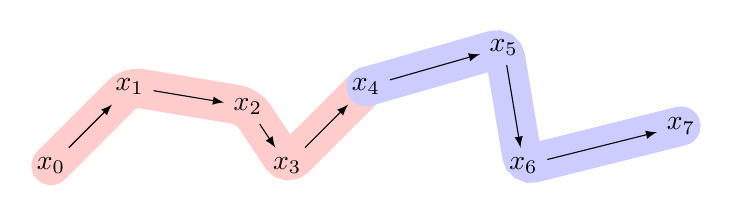
\begin{tikzpicture}
				\coordinate (a0) at (0,0);
				\coordinate (a1) at (1,1);
				\coordinate (a2) at (2.5,.75);
				\coordinate (a3) at (3,0);
				\coordinate (a4) at (4,1);
				\coordinate (a5) at (5.75,1.5);
				\coordinate (a6) at (6,0);
				\coordinate (a7) at (8,.5);
				%
				\draw[red!20,line width=5mm, rounded corners, cap=round] (a0) -- (a1) -- (a2) -- (a3) -- (a4);
				\draw[blue!20,line width=5mm, rounded corners, cap=round] (a4) -- (a5) -- (a6) -- (a7);
				%
				\foreach \i in {0,...,7}
				\node (e\i) at (a\i) {$x_\i$};
				\foreach \i in {0,...,6}{
						\edef\ipp{\fpeval{\i + 1}}
						\draw[-latex] (e\i) -- (e\ipp);
					}
			\end{tikzpicture}
		\end{center}
		\caption{Composizione di due morfismi \((e_1,e_2,e_3,e_4)\) e \((f_1,f_2,f_3)\) in \(\bfF[\ctG]\).}
		\label{fig:enter-label}
	\end{figure}
\end{example}
Dopo questa digressione veniamo a due esempi più elaborati, ma molto `concreti', di categorie dove gli oggetti sono numeri naturali:
\begin{hExample}[La categoria dei circuiti digitali]{tech}\label{ex_cat_circuiti}\index{Categoria!--- dei circuiti}
	La categoria \(\ctCirc\) ha
	\begin{itemize}
		\item per oggetti i numeri naturali \(0,1,2,\dots\);
		\item l'insieme dei morfismi \(\ctCirc(m,n)\) consiste dell'insieme delle funzioni \(\bbB^n\to \bbB^m\), dove \(\bbB=\{0,1\}\) è l'insieme dei \emph{Booleani}\footnote{L'insieme \(\bbB\) può essere interpretato come: l'insieme degli interi positivi modulo 2, l'insieme degli stati di un singolo bit di informazione; l'insieme \{sì, no\} delle risposte a una domanda; l'insieme \(\{-1,1\}\) dei \emph{segni} assunti dagli elementi dell'immagine di una funzione reale, l'insieme \{acceso, spento\} degli stati di un interruttore, eccetera.} e \(\bbB^0\defeq \{*\}, \bbB^{n+1}\defeq \bbB^n\times \bbB\) sono i prodotti cartesiani iterati di \(\bbB\) con sé stesso.
	\end{itemize}
	Si noti che ogni funzione Booleana \(f : \bbB^n\to\bbB^m\) risulta dal `prodotto' di \(m\) funzioni Booleane \emph{semplici} \(\tup fm, : \bbB^n\to\bbB\), di modo che
	\[f(\tup xn,)=(f_1(\tup xn,),\dots,f_m(\tup xn,)).\]
	Tra le funzioni Booleane semplici ci sono certamente le proiezioni canoniche \(\pi_{n,i} = \pi_i : \bbB^n\to\bbB :(\tup xn,)\mapsto x_i\), con le quali è possibile caratterizzare le \(f_i\) su menzionate: \(f_i = \pi_i\cmp f\); è anche possibile definire la mappa diagonale \(\Delta_m:\bbB\to\bbB^m\) come
	\[\Delta_m : x\mapsto (x,\dots,x)\quad m\text{ volte}\]
	cioè mediante le \(m\) funzioni semplici identità \(x\mapsto x\).

	Sull'insieme dei Booleani è possibile definire le operazioni logiche elementari di disgiunzione, congiunzione e negazione logica, che è possibile rappresentare graficamente con i seguenti diagrammi o `porte' logiche (note a qualsiasi ingegnere elettronico)
	\[\begin{circuitikz}
			\node[font=\tiny, xshift=-3cm, or port, fill=gray!10] (4,0) (or) {\(\text{OR}\)};
			\node[font=\tiny, and port, fill=gray!10] (0,0) (and) {\!\!\(\text{AND}\)};
			\node[font=\tiny, xshift=2.5cm, not port, fill=gray!10] (0,0) (not) {\!\!\(\text{NOT}\)};
		\end{circuitikz}\]
	\`E possibile comporre in serie le porte logiche, componendo i morfismi che esse rappresentano, e giustapporle in parallelo, allo stesso modo in cui è possibile considerare circuiti elettrici in serie e in parallelo per costruire strutture complesse come:
	\[
		\begin{circuitikz}[fill=gray!10]
			\draw (0,3) node[american and port] (A) {};
			\draw (A.out) -- ++(0.5,0) node[american or port,
				number inputs=2, anchor=in 1] (B) {};
			\draw (0,1.5) node[american or port] (C) {};
			\draw (C.out) |- (B.in 2);
			\draw (B.out) -- ++(.5,0) node[american not port,anchor=in 1] (D) {};
		\end{circuitikz}
	\]
	che rappresenta la funzione Booleana semplice
	\[(x,y,z,w)\mapsto \lnot((x\land y)\lor(z\lor w)).\]
\end{hExample}
Vale il seguente teorema:
\begin{theorem}\label{circ_thm}\index{Funzione Booleana}
	Ogni funzione Booleana semplice \(f :\bbB^n\to\bbB\) è esprimibile come composizione in serie e in parallelo di: proiezioni, mappe diagonali, congiunzioni e negazioni logiche.
\end{theorem}
Una maniera alternativa di esprimere questo risultato è affermare che l'insieme \(\{\text{AND},\text{OR}\}\) è \emph{funzionalmente completo} (o un \emph{insieme universale}) per il calcolo di porte logiche. Per una dimostrazione, si veda \cite[Teorema 1.4]{Crama2011}. In termini categoriali, stiamo affermando che un certo insieme di morfismi genera, insieme alle \(\pi_{n,1},\dots,\pi_{n,n}\) e \(\Delta_n\) per ogni \(n\ge 0\), l'intera categoria mediante le operazioni di prodotto e composizione.

Il capitolo \ref{chap_limiti_colimiti} e in particolare la nozione di prodotto, introdotta in \ref{chap_limiti_colimiti}, renderanno chiaro il ruolo fondamentale delle mappe \(\Delta_n,\tup{\pi}n,\) in questa e molte altre costruzioni.
\subsection{Categorie come universi}\label{ssec:categorie_universi}
Proseguiamo con degli esempi di categorie grandi, che giustificano l'intuizione per le categorie come `universi del discorso matematico', ossia come classi i cui elementi sono collegati da relazioni reciproche. L'esempio fondamentale per tutta la sezione è \ref{ex_cat_insiemi}, la categoria di insiemi e funzioni. Usando questa categoria \(\ctSet\) come esempio paradigmatico, è possibile costruire
\begin{itemize}
	\item categorie di strutture algebriche (gruppi, anelli, algebre su un campo di base\dots); esempi di queste categorie sono \ref{ex_cat_monoidi}, e in generale \ref{ex_cat_sigma_strutture};
	\item categorie di strutture topologiche/ordinate (spazi topologici, insiemi parzialmente ordinati); esempi di queste categorie sono \ref{po_wo_to}, \ref{ex_cat_top};
\end{itemize}
e insieme a queste, molte altre. Esiste una dicotomia forte tra queste due classi di categorie, che sarà possibile apprezzare una volta introdotti più strumenti.

\`E tuttavia estremamente importante notare che
\begin{quote}
	Non tutte le categorie larghe si possono vedere come categorie di insiemi strutturati. Ad esempio, la categoria di \ref{ex_cat_hotop} non ha la proprietà di essere \emph{concreta} (si veda \ref{ssec:categorie_strutture}, \ref{def_costrutto}).
\end{quote}
\begin{example}[Insiemi e relazioni]\label{ex_cat_rels}\index{Categoria!--- delle relazioni}
	La categoria \(\ctRel\) ha
	\begin{itemize}
		\item per oggetti gli insiemi, denotati con le lettere \(A,B,C,\dots\);
		\item per morfismi da \(A\) verso \(B\) tutte le \emph{relazioni} \(R\subseteq A\times B\), ossia i sottoinsiemi del prodotto cartesiano \(A\times B\).
	\end{itemize}
	Una relazione \(R\subseteq A\times B\) e una relazione \(S\subseteq B\times C\) si compongono nella relazione \(S\cmp R\) definita da
	\[(a,c)\in S\cmp R\iff \exists (b\in B) : ((a,b)\in R)\land ((b,c)\in S).\]
	Con questa definizione, si può mostrare che \(T\cmp(S\cmp R)=(T\cmp S)\cmp R\) e che la relazione diagonale \(\{(a,a)\mid a\in A\}\subseteq A\times A\) (ovvero la relazione \(a\,\Delta\,a'\iff a=a'\)) funge da elemento identità per la composizione così definita.
\end{example}
Nell'esempio appena fatto, l'ordine in cui si scrivono i fattori di un prodotto cartesiano è importante, perché se \(R : A\to B\) è una relazione, vogliamo che \(A\) ne sia il dominio, e \(B\) il codominio. \`E però vero che gli insiemi \(A\times B\) e \(B\times A\) sono in biiezione canonica, e quindi si potrebbe pensare di definire una categoria \(\ctRel'\) con gli stessi oggetti di \(\ctRel\), ma con morfismi da \(A\) verso \(B\) le relazioni \(R\subseteq B\times A\). In effetti, questa è la categoria opposta \(\ctRel^\op\) di \(\ctRel\) (si veda \ref{def_cat_opp}), e tra \(\ctRel^\op\) e \(\ctRel\) esiste un isomorfismo (si veda \ref{rel_autoduale}).
\begin{remark}\label{klext_delle_relazioni}\index{Relazione}\index{Relazione!estensione di ---}
	Ogni relazione \(R : A\to B\) induce una funzione \(R^* : \pow B\to \pow A\) nel modo che segue: un sottoinsieme \(U\subseteq B\) viene mandato in \(R^*U:=\{x\in A\mid \forall u\in U.(x,u)\in R\}\). In effetti, esiste una analoga funzione \(R_* : \pow A\to \pow B\), definita da \((V\subseteq A) \mapsto R_*V:= \{y\in B\mid \forall v\in V.(v,y)\in R\}\), e tra le due funzioni \(R^*, R_*\) sussiste la relazione
	\[V\subseteq R^*U \iff U\subseteq R_*V\label{aggiunti_in_disguise}\]
	dal momento che il lato sinistro è equivalente a \(\forall v\in V.\forall u\in U.(v,u)\in R\) e il lato destro a \(\forall u\in U.\forall v\in V.(v,u)\in R\). Nel capitolo \ref{cap_aggiunti} questo sarà un esempio elementare di una nozione importante, quella di \emph{aggiunzione} tra due categorie.
\end{remark}
\begin{remark}\label{diff_pres_cat_rel}
	L'osservazione precedente permette una differente presentazione per la categoria \(\ctRel\): gli oggetti di \(\ctRel\) sono ancora gli insiemi, ma una relazione \(R\subseteq X\times Y\) viene ora presentata come una \emph{funzione}
	\[\dmFun RX{\pow Y}\]
	definita mandando \(x\in X\) nell'insieme \(Rx = \{y\in Y\mid xRy\}\), e una tale relazione induce un'unica funzione \(\hat R : \pow X\to \pow Y\) definita da \(\hat R(U) = \bigcup_{x\in U}Rx = \{y\in Y\mid \exists x\in U,\, y\in Rx\}\), chiamata \emph{estensione di Kleisli} di \(R\) (il capitolo \ref{}, sulle monadi, chiarirà questa terminologia).

	La composizione di due relazioni \(R\subseteq X\times Y\) e \(S\subseteq Y\times Z\) è data dalla composizione \emph{di funzioni} \(\hat S\cmp R\), cioè
	\[
		x \mapsto \hat S(Rx) = \{z\in Z\mid \exists y\in Rx,\, ySz\}.
	\]
	Le proprietà generali di una estensione di Kleisli, che permettono di dimostrare che la definizione data soddisfa gli assiomi di categoria, sono le seguenti (tutte di facile dimostrazione, che lasciamo per esercizio):
	\begin{enumtag}{ek}
		\item \label{ek_1} per ogni insieme \(A\), esiste una \emph{relazione identica} \(\eta_A : A\to \pow A\), e \(\hat\eta_A\) è l'identità di \(\pow A\);
		\item \label{ek_2} se \(R : B\to \pow A\) è una relazione, allora \(\hat R\cmp \eta_B = R : B \to\pow A\);
		\item \label{ek_3} se \(R : B\to \pow A\) e \(S : C\to \pow B\) sono due relazioni, allora \(\hat S\cmp \hat R = \hat{S\cmp R} : C\to \pow A\).
	\end{enumtag}
\end{remark}
\begin{example}[Insiemi e funzioni]\label{ex_cat_insiemi}\index{Categoria!--- degli insiemi}
	\index{Categoria!--- degli insiemi finiti|see {--- degli insiemi}}\index{Insieme}
	La categoria \(\ctSet\) ha
	\begin{itemize}
		\item per oggetti gli insiemi, denotati con le lettere \(A,B,C\dots\);
		\item per morfismi da \(A\) verso \(B\) tutte le funzioni \(f : A\to B\), ossia tutte le relazioni \(F\subseteq A\times B\) con la proprietà che per ogni \(a\in A\) esiste un unico \(b\in B\) tale che \((a,b)\in F\) o, più formalmente, \(F\cap(\{a\}\times B)\) è un singoletto; l'elemento \(b\) in questione si denota \(f(a)\) o \(fa\) e l'insieme \(F = \{(a,fa)\mid a\in A\}\) è il \emph{grafico} o \emph{supporto} della funzione. Queste relazioni sono \emph{totali} (perché sono definite sull'intero dominio \(A\)) e \emph{a valore singolo}.
	\end{itemize}
	Due funzioni \(f : A\to B\), \(g : B\to C\) si compongono alla maniera delle relazioni (e la composizione è ancora una funzione, poiché l'intersezione \((G\cmp F)\cap (\{a\}\times C)\) consta del singoletto \(\{g(f(a))\}\)).

	La relazione diagonale è infine la (relazione sottostante alla) funzione identità.
\end{example}
Evidentemente, possiamo restringerci a considerare la categoria dei soli insiemi \emph{finiti} (così come la categoria \(\ctFRel\) delle relazioni tra insiemi finiti, che la contiene propriamente). Questo è il primo degli esempi motivanti fatti ad inizio capitolo, e in un senso evidente (che sarà precisato dalla definizione \ref{def_subcat}), \(\ctFRel\) è una \emph{sottocategoria} di \(\ctRel\) (e \(\ctFin\) è una sottocategoria di \(\ctSet\), che a sua volta è una sottocategoria di \(\ctRel\), sebbene in un modo non completamente banale).
\begin{example}[Categoria delle matrici in \(\bbF\)]\label{ex_cat_matrici}\index{Categoria!--- delle matrici}
	Per ogni anello con divisione \(\bbF\), posiamo definire la categoria \(\ctMat\) delle \emph{matrici a componenti in \(\bbF\)} come quella che ha
	\begin{itemize}
		\item per oggetti i numeri naturali \(0,1,2,\dots\);
		\item per morfismi \(n\to m\) le matrici con \(m\) righe ed \(n\) colonne a coefficienti in \(\bbF\), ossia:
		      \[\ctMat(n,m) = \matrici mn\bbF = \text{Lin}_{\bbF}(\bbF^n,\bbF^m)\]
		      dove \(\bbF^n:=\bbF \times\dots\times\bbF\) è il prodotto cartesiano iterato di \(\bbF\) con sé stesso \(n\) volte (quindi \(\bbF^0\) contiene il solo vettore nullo), e \(\text{Lin}_{\bbF}(\bbF^n,\bbF^m)\) è l'insieme delle funzioni \(\bbF\)-lineari \(\bbF^n\to\bbF^m\) (che scegliendo su dominio e codominio le basi canoniche, si identifica alle matrici a componenti in \(\bbF\) di taglia \(m\times n\)).
	\end{itemize}
	La composizione è il prodotto di matrici: se \(A : n\to m\) e \(B : m\to p\) sono matrici di entrate \((A_{ij}\mid 1\le i\le m,1\le j\le n)\) e \((B_{rs}\mid 1\le r\le p,1\le s\le m)\), la loro composizione \(BA : n\to p\) è la matrice \(BA\in \matrici pn\bbF\) definita da \((BA)_{ij} = \sum_{k=1}^m B_{ik}A_{kj}\).

	Questa operazione di composizione, come ricorda chiunque abbia studiato l'algebra lineare, è associativa, e la matrice identità \(I_n\in \matrici nn\bbF\) ne è l'elemento identità.
\end{example}
\begin{remark}\index{Vect@\(\ctVect\)}
	La categoria degli spazi vettoriali e mappe lineari, introdotta indirettamente in \ref{varie_categorie_nella_pratica}, e la categoria \(\ctMat\) ora definita, sono collegate in un senso preciso che sarà chiaro introducendo la nozione di \emph{scheletro} di una categoria in \ref{def_scheletro}: \(\ctMat\) si ottiene da \(\ctVect\) scegliendo un solo oggetto per ogni dimensione (dato che ogni \(\bbF\)-spazio vettoriale \(V\) di dimensione finita su \(\bbF\) è isomorfo ad un oggetto di \(\ctMat\)).
\end{remark}
Questo appena fatto è il secondo degli esempi motivanti fatti ad inizio capitolo.
\index{Categoria!--- di strutture algebriche}
\begin{example}\label{ex_cat_monoidi}\index{Omomorfismo!---di monoidi}
	Dati due monoidi \(M\) e \(N\), un \emph{omomorfismo di monoidi} \(f:M\to N\) è una funzione \(f:M\to N\) tale che
	\begin{itemize}
		\item \(f(e) = e\), cioè mappa l'elemento neutro di \(M\) in quello di \(N\);
		\item \(f(m\cdot m')=f(m)\cdot f(m')\) per ogni \(m,m'\in M\), cioè rispetta la moltiplicazione.
	\end{itemize}
	In particolare, se \(M\) ed \(N\) sono gruppi, un omomorfismo di monoidi è esattamente un omomorfismo di gruppi.
	Come si può facilmente verificare, l'identità su un monoide è un omomorfismo, e la composizione di omomorfismi è un omomorfismo.
	\begin{itemize}
		\item I monoidi e gli omomorfismi di monoidi formano la categoria \(\ctMon\).
		\item I gruppi e gli omomorfismi di gruppo formano la categoria \(\ctGrp\).
	\end{itemize}
\end{example}
L'idea da trattenere dopo questi primi esempi è che tutte le categorie di insiemi con operazioni che soddisfano, eventualmente, delle equazioni, forma una categoria; sebbene a volte non sia una questione banale scegliere la `giusta' nozione di omomorfismo tra strutture, ci affidiamo alla competenza che gli studi anteriori hanno dato a chi legge nel capire che, anche quando non abbiamo definito precisamente oggetti e morfismi, ci riferiamo alle categorie di strutture algebriche con le loro scelte `ovvie' di omomorfismo come funzione che rispetta (tutta) la struttura algebrica. Un'utile intuizione a riguardo è che in qualsiasi circostanza dove una classe di strutture possieda una nozione di omomorfismo che preserva la specifica di quella struttura, e tale che
\begin{itemize}
	\item l'identità è un omomorfismo;
	\item la composizione di due omomorfismi è ancora un omomorfismo;
\end{itemize}
si riesce a definire la classe degli oggetti e dei morfismi di una categoria.

L'\emph{algebra universale} si occupa di rendere preciso il concetto di `insieme dotato di operazioni', codificando una struttura algebrica mediante una \emph{funzione di arietà}:\footnote{Le parole \emph{arietà}, così come \emph{nullario} e \emph{unario} e \(n\)-ario (ma non binario, ternario, quaternario, etc.) sono retroformazioni che il lessico matematico ha introdotto a partire dal suffisso latino \emph{-\={a}rius, -\=aria, -\=arium}, usato per formare aggettivi a partire da nomi o numerali. Una operazione `\(n\)-aria' accetta \(n\) argomenti a dominio.} innanzitutto, si ricordi che una operazione \(n\)-aria su un insieme \(X\) consta di una funzione \(X\times X\times\dots\times X \to X\) dove il prodotto cartesiano è fatto \(n\) volte.
\begin{example}\label{ex_cat_sigma_strutture}\index{Categoria!---}
	Una \emph{segnatura algebrica} consiste di una coppia \((\Omega, a)\) dove \(\Omega\) è un insieme, e \(a : \Omega \to \bbN\) è una funzione detta \emph{funzione di arietà} che associa a ogni elemento \(\omega \in \Omega\) la sua arietà \(a(\omega)\ge 0\). Un \emph{modello} per una segnatura algebrica \((\Omega,a)\) consiste di un insieme \(X\) e di una funzione \(f_\bullet\) che associa a ogni \(\omega\in\Omega\) una operazione \(f_\omega : X^{a(\omega)} \to X\) di arietà \(a(\omega)\).

	Fissata una segnatura algebrica \((\Omega,a)\) possiamo definire la categoria \(\ctMod(\Omega,a)\) dei suoi modelli come segue:
	\begin{itemize}
		\item gli oggetti di \(\ctMod(\Omega,a)\) sono precisamente i modelli \((X,f_\bullet)\) di \((\Omega,a)\);
		\item fissati due modelli \((X,f_\bullet), (Y,g_\bullet)\) un \emph{omomorfismo} di modelli è una funzione \(h : X\to Y\) con la proprietà che per ogni \(\omega\in\Omega\) si abbia l'uguaglianza
		      \[h(f_\omega(\tup x{a(\omega)},)) = g_\omega(\tup {hx}{a(\omega)},)\]
		      o in termini diagrammatici, il seguente diagramma commuta.
		      \[
			      \begin{tikzcd}
				      X^{a(\omega)} \ar{r}{h^{a(\omega)}} \ar[d, "f_\omega"'] & Y^{a(\omega)} \ar{d}{g_\omega} \\
				      X \ar[r, "f"']& Y
			      \end{tikzcd}
		      \]
	\end{itemize}
\end{example}
\`E un esercizio tedioso nella manipolazione delle tuple ordinate, ora, dimostrare che gli assiomi di categoria sono tutti soddisfatti. Un esercizio analogamente tedioso è di trovare segnature algebriche opportune che esprimono le categorie dei gruppi, dei monoidi, degli anelli e degli spazi vettoriali ecc.\ come esempi particolari di categorie di modelli di una segnatura algebrica.\footnote{Tedioso, e a volte non proprio banale: ad esempio, come si descrivono le operazioni di moltiplicazione per scalare in uno spazio vettoriale usando la definizione di segnatura algebrica? Si noti anche che la richiesta che un omomorfismo di modelli rispetti \emph{tutti} gli elementi della segnatura a volte è ridondante: ogni omomorfismo di gruppi \(f : G\to H\) manda l'identità del dominio nell'identità del codominio perché \(f(e_G)\) deve essere un elemento idempotente di \(H\), e preserva gli inversi come corollario.}
\begin{remark}\label{varie_categorie_nella_pratica}\index{Categoria!---e di strutture algebriche}
	Categorie di modelli come in \ref{ex_cat_sigma_strutture} sono tra le più comuni da considerare nella pratica matematica: i monoidi e i loro omomorfismi, i gruppi e i loro omomorfismi (tra essi, la sottocategoria dei gruppi abeliani), gli anelli e i loro omomorfismi (tra essi, la sottocategoria degli anelli commutativi), gli spazi vettoriali su un campo \(k\) e le funzioni \(k\)-lineari, formano tutte esempi di categorie, che denotiamo con \(\ctMon\), \(\ctGrp\), \(\ctAb\), \(\ctRing\), \(\ctcRing\), \(\ctVect[k]\),\dots
\end{remark}
\begin{example}[Categoria dei multidigrafi]\label{ex_cat_grafi}\index{Categoria!--- dei grafi}
	Questo esempio rende precise alcune osservazioni fatte in precedenza, \ref{ex_cat_doppiafreccia} e \ref{ex_cat_libera}. La categoria \(\ctdGph\) dei grafi è così definita:
	\begin{itemize}
		\item gli oggetti di \(\ctdGph\) sono i grafi, o più precisamente i \emph{multidigrafi}: un (multidi)grafo \(\ctG = (E,V,s,t)\) consiste di una coppia di insiemi \(E,V\) dotati di due funzioni \(s,t : E\toto V\) che associano ad ogni \emph{lato} \(e\in E\) una coppia ordinata di \emph{vertici} \(s(e),t(e)\in V\) detti il suo dominio o \emph{source} e il suo codominio o \emph{target}.
		\item Un omomorfismo di (multidi)grafi \((f_E,f_V) : (E,V,s,t)=\ctG\to\ctG'= (E', V',s',t')\) consiste in una coppia di funzioni \(f_E, f_V\) tali che
		      \begin{gather*}
			      s'\cmp f_E = f_V\cmp s\\
			      t'\cmp f_E = f_V\cmp t
		      \end{gather*}
		      o in termini diagrammatici, tali che i due quadrati seguenti siano commutativi,
		      % https://q.uiver.app/#q=WzAsOCxbMCwwLCJFIl0sWzAsMSwiViJdLFsxLDAsIkUnIl0sWzEsMSwiViciXSxbMiwwLCJFIl0sWzMsMCwiRSciXSxbMiwxLCJWIl0sWzMsMSwiViciXSxbMCwyLCJmX0UiXSxbMiwzLCJzJyJdLFsxLDMsImZfViIsMl0sWzAsMSwicyIsMl0sWzQsNSwiZl9FIl0sWzYsNywiZl9WIl0sWzUsNywidCciXSxbNCw2LCJ0IiwyXV0=
		      \[\begin{tikzcd}
				      E & {E'} & E & {E'} \\
				      V & {V'} & V & {V'}
				      \arrow["{f_E}", from=1-1, to=1-2]
				      \arrow["{s'}", from=1-2, to=2-2]
				      \arrow["{f_V}"', from=2-1, to=2-2]
				      \arrow["s"', from=1-1, to=2-1]
				      \arrow["{f_E}", from=1-3, to=1-4]
				      \arrow["{f_V}"', from=2-3, to=2-4]
				      \arrow["{t'}", from=1-4, to=2-4]
				      \arrow["t"', from=1-3, to=2-3]
			      \end{tikzcd}\]
		      cosicché \((f_E,f_V)\) commutano con le funzioni di source e target.
	\end{itemize}
	Si noti che questo significa che questo impone precisamente che per ogni \(e\in E\), \(f_E(e)\) sia un lato in \(E'\) di vertici \(f_V(se), f_V(te)\) rispettivamente.
\end{example}
Evidentemente, possiamo scrivere \(e : x\to y\) per denotare in maniera compatta il fatto che \(e \in E\) è un lato tale che \(se=x,te=y\); allora un omomorfismo di multidigrafi è tale che se \(e : x\to y\), allora \(f_Ee : f_Vx\to f_Vy\).
\begin{example}[Categoria dei grafi]\label{ex_cat_grafi_nondiretti}\index{Categoria!--- dei grafi non diretti}
	In maniera simile possiamo definire la categoria \(\ctGph\) dei grafi non diretti; un grafo non diretto è un insieme \(V\) di vertici, su cui sia definita una relazione \(E\subseteq V\times V\), simmetrica e irriflessiva (cioè \(\forall v\in V.(v,v)\notin E\)).

	Un omomorfismo di grafi non diretti è una funzione tra i vertici \(f_V : V\to V'\) compatibile con le relazioni \(E,E'\): se \((u,v)\in E\), allora \((fu,fv)\in E'\).
\end{example}
\begin{example}\label{ex_cat_ordini}\index{Categoria!--- di insiemi ordinati}
	\index{Preordine}
	Si ricordi da \ref{prelim_def_preset} che un \emph{insieme preordinato} è un insieme \(P\) dotato di una relazione riflessiva e transitiva \(\le\) che si dice la \emph{(relazione d')ordine} su \(P\); una funzione \(f : (P,\le)\to (Q,\preceq)\) si dice \emph{monotòna} o si dice che \(f\) \emph{preserva l'ordine} se vale
	\[\forall x,y(x\le y\Rightarrow fx\preceq fy).\]

	La categoria \(\ctPOrd\) ha per oggetti e morfismi gli insiemi preordinati e le funzioni monotòne. Chiaramente, l'identità \(\id_P : (P,\le)\to (P,\le)\) è una funzione monotòna, e la composizione di due funzioni monotòne resta monotòna.

	\`E tuttavia importante che l'ordine su \(P\) sia \emph{lo stesso} affinché l'identità sia monotòna: infatti, ogni insieme \(P\) può essere dotato dell'ordine \emph{banale} (dove \(x \mathrel{\le^\delta} y\) se e solo se \(x=y\)) e dell'ordine \emph{caotico} (dove \(x\mathrel{\le^\chi} y\) per ogni \(x,y\in P\)). Se \(P\) ha almeno due elementi, la funzione identità \((P,\le^\chi)\to (P,\le^\delta)\) non è, chiaramente, monotòna.
\end{example}
\begin{remark}[po, wo e to]\label{po_wo_to}\index{Ordine parziale}\index{Ordinale}
	Una sottoclasse importante di preordini si ottiene imponendo che \(\le\) sia una relazione antisimmetrica; in tal caso il preordine \((P,\le)\) si dice un \emph{insieme parzialmente ordinato} (in inglese, \emph{p}artially \emph{o}rdered \emph{set} o brevemente \emph{poset}). La categoria \(\ctPos\) ha per oggetti i poset e per morfismi le stesse funzioni monotòne di \ref{ex_cat_ordini}.

	Un'altra sottocategoria importante di \(\ctPOrd\) è quella degli insiemi \emph{totalmente ordinati} o \emph{toset}, dove tutti gli elementi sono confrontabili tra loro:
	\[\forall x,y\in P.((x\le y)\lor (y\le x));\]
	da ultimo, una ulteriore sottocategoria importante di \(\ctPOrd\) è quella degli insiemi \emph{bene ordinati} (in inglese, \emph{w}ell \emph{o}rdered sets, o brevemente \emph{wosets}), dove ogni sottoinsieme non vuoto ammette un elemento minimo. Se \((P,\le)\) è un woset, si dice anche che \(P\) è un \emph{buon ordine} rispetto a \(\le\).
\end{remark}
\begin{example}\label{ex_cat_ordinali}\index{Categoria!--- degli ordinali}
	Ricordiamo che un insieme \(X\) si dice \emph{transitivo} se una qualsiasi delle seguenti condizioni equivalenti è soddisfatta:
	\begin{itemize}
		\item \(x\in X\Rightarrow x\subseteq X\);
		\item \(X\subseteq \pow X\);
		\item \(\bigcup X\subseteq X\).
	\end{itemize}
	Un insieme \(X\) si dice un \emph{ordinale} se è transitivo e se ogni sottoinsieme non vuoto \(S\subseteq X\) ammette un elemento \(\in\)-minimo, cioè se \(X\) è bene ordinato dalla relazione \(\in\).

	La categoria \(\ctOrd\) ha per oggetti gli ordinali e per morfismi \(X\to Y\) le funzioni monotòne.
\end{example}
L'importanza della categoria degli ordinali sarà più evidente quando in \ref{sec_funtori} introdurremo la definizione di funtore. Per il momento, ci limitiamo ad alcune osservazioni.
\begin{remark}\label{rmk_delta_e_deltaPlus}\index{Ordinale!--- finito}\index{Categoria!--- dei simplessi}
	Se \([n]=\{\iter[0] n\}\) è un insieme finito, l'ordinamento \(\{\iter[0][<]n\}\) lo rende un woset nel senso di \ref{po_wo_to}, e quindi \(\Delta[n]\) è in maniera naturale un oggetto di \(\ctPos\), ma anche di \(\ctOrd\); insieme alle funzioni monotòne tra questi insiemi finiti, ciò identifica la sottocategoria di \(\ctOrd\) generata da tutte le catene generiche \(\Delta[n]\) di \ref{ex_cat_catena} con la sottocategoria \(\ctFOrd\) di tutti gli ordinali finiti e non vuoti.
	\begin{itemize}
		\item Una notazione alternativa e più comune, mutuata dalla topologia algebrica, per \(\ctFOrd\)	è \(\bsDelta\) (la lettera greca delta maiuscola), che viene chiamata la categoria dei \emph{simplessi}.
		\item Per la categoria di \emph{tutti} gli ordinali, anche quello vuoto, si usa la notazione \(\bsDelta_+\), che viene chiamata la categoria dei \emph{simplessi aumentati}.
	\end{itemize}
\end{remark}
\begin{figure}[h]
	\begin{center}
		\begin{tikzpicture}[
				x=4em, y=4em,
				wrap/.style={fill=black!5, rounded corners},
				edge/.style={-latex},
				0simplex/.style={font=\scriptsize,inner sep=2pt},
			]
			\begin{scope}[xshift=0em,yshift=0.433*5em]
				\node[0simplex] (0D0) at (0.0,0) {0};
			\end{scope}
			\begin{scope}[xshift=4em,yshift=0.433*5em]
				\node[0simplex] (1D0) at (0.0,0) {0};
				\node[0simplex] (1D1) at (1.0,0) {1};
				\draw[edge, ibmMagenta] (1D0) -- (1D1);
			\end{scope}
			\begin{scope}[xshift=13em]
				\node[0simplex] (2D0) at (0.0,0) {0};
				\node[0simplex] (2D1) at (1.0,0) {1};
				\node[0simplex] (2D2) at (0.5,0.866) {2};
				\draw[edge, ibmMagenta] (2D0) -- (2D1);
				\draw[edge] (2D0) -- (2D2);
				\draw[edge, ibmMagenta] (2D1) -- (2D2);
			\end{scope}
			\begin{scope}[xshift=22em]
				\node[0simplex] (3D0) at (0.0,0) {0};
				\node[0simplex] (3D1) at (1.0,0) {1};
				\node[0simplex] (3D2) at (0.5,0.866) {2};
				\node[0simplex] (3D3) at (0.5,0.3) {3};
				\draw[edge,ibmMagenta] (3D0) -- (3D1);
				\draw[edge] (3D0) -- (3D2);
				\draw[edge,ibmMagenta] (3D1) -- (3D2);
				\draw[edge] (3D0) -- (3D3);
				\draw[edge] (3D1) -- (3D3);
				\draw[edge,ibmMagenta] (3D2) -- (3D3);
			\end{scope}
			\begin{scope}[on background layer]
				\path node[wrap, fit=(0D0)] (W0) {};
				\path node[wrap, fit=(1D0)(1D1)] (W1) {};
				\path node[wrap, fit=(2D0)(2D1)(2D2)] (W2) {};
				\path node[wrap, fit=(3D0)(3D1)(3D2)(3D3)] (W3) {};
				\node [below=2.5em of W0] (L) {$\Delta[0]$};
				\node at (L -| W1) {$\Delta[1]$};
				\node at (L -| W2) {$\Delta[2]$};
				\node at (L -| W3) {$\Delta[3]$};
			\end{scope}
		\end{tikzpicture}
	\end{center}
	\caption{Le categorie \(\Delta[0], \dots,\Delta[3]\) già viste in \ref{ex_cat_catena}, con le loro \emph{spine} in evidenza; la spina di un simplesso è la catena di frecce \(0\to 1\to\cdots\to n\) che genera, per composizione, tutte le altre frecce di \(\Delta[n]\).}
	\label{fig:spines}
\end{figure}
\begin{hRemark}[Combinatoria della categoria \(\ctFOrd\)]{skip}\label{rmk_combinatoria_simplessi}\index{Categoria!--- dei simplessi}
	La categoria \(\bsDelta\) possiede una sottoclasse di morfismi che generano tutti gli altri per composizione. Tra tutte le mappe monotòne \(f : [n]\to [m]\) in \(\bsDelta\) possiamo distinguere le \(n+1\) funzioni \emph{iniettive} \(\delta_n^i : [n-1]\mono [n]\) che evitano l'elemento \(i=\iter[0]n\), e le \(n+1\) funzioni \emph{suriettive} \(\sigma_n^j : [n+1]\epi [n]\) che assumono due volte il valore  \(j=\iter[0]m\):
	\[
		\delta_n^i(k) =
		\begin{cases}
			k,   & k < i    \\
			k+1, & k \geq i
		\end{cases}
		\quad \quad
		\sigma_n^j (k) =
		\begin{cases}
			k,   & k \leq j \\
			k-1, & k > j
		\end{cases}
		\quad \text{per} \quad 0 \leq j\leq n.
	\]
	\index{Insieme simpliciale}\index{Insieme!--- simpliciale}
	Per ogni \(n\ge 0\), \(\{\delta_n^0,\dots,\delta_n^{n+1}\}\) sono dette le \emph{cofacce} di \([n]\), e \(\{\sigma_n^0,\dots, \sigma_n^n\}\) le \emph{codegenerazioni} di \([n]\). Raffiguriamo alcune mappe di cofaccia e codegenerazione in \autoref{fig:cofa} e \ref{fig:code}. Tali funzioni soddisfano le seguenti relazioni, dette \emph{identità cosimpliciali}:
	\begin{gather*}
		\delta_n^j \cmp \delta_{n-1}^i = \delta_n^i \cmp \delta_{n-1}^{j-1}, \quad i < j\\
		\sigma_n^j \cmp \sigma_n^i = \sigma_n^i \cmp \sigma_n^{j+1}, \quad i \leq j\\
		\sigma_n^j \cmp \delta_n^i =
		\begin{cases}
			\delta_n^i \cmp \sigma_n^{j-1}, & i < j      \\
			\id,                            & i = j, j+1 \\
			\delta_n^{i-1} \cmp \sigma_n^j, & i > j+1.
		\end{cases}
	\end{gather*}
	Ogni freccia di \(\Hom\bsDelta([n],[m])\) si può scrivere, in maniera essenzialmente unica, come composizione di alcune mappe di codegenerazione, seguite da alcune mappe di cofaccia; l'idea è di fattorizzare \(f\) lungo la sua immagine (dotata dell'ordine indotto),
	\[\xymatrix{
			[n]\ar[rr]^f\ar[dr]_e &&	[m] \\
			& \im(f) \ar[ur]_m
		}\]
	e conseguentemente immergere quest'ultima nel codominio. La funzione suriettiva \(e\) è composizione di codegenerazioni (precisamente quelle determinate dai valori che \(f\) assume molteplici volte), e la funzione iniettiva \(m\) è composizione di alcune cofacce (precisamente quelle determinate dai valori che \(f\) non assume).
\end{hRemark}
\begin{figure}
	\begin{center}
		\begin{tikzpicture}[x=.5cm]
			\tikzset{
				fitbg/.style={inner sep=0pt, fill=gray!50, opacity=0.5}
			}
			\drawChain{3}[up]
			\begin{pgfonlayer}{background}
				\node[fitbg,fit=(0up)(3up)] {};
			\end{pgfonlayer}
			\begin{scope}[yshift=-1cm]
				\drawChain{4}[down]
				\begin{pgfonlayer}{background}
					\node[fitbg,fit=(1down)(4down)] {};
				\end{pgfonlayer}
			\end{scope}
			\foreach \i/\j in {0/1,1/2,2/3,3/4}
			\draw[-latex] (\i up) -- (\j down);
			\begin{scope}[xshift=3cm]
				\drawChain{3}[up]
				\begin{pgfonlayer}{background}
					\node[fitbg,fit=(0up)] {};
					\node[fitbg,fit=(1up)(3up)] {};
				\end{pgfonlayer}
				\begin{scope}[yshift=-1cm]
					\drawChain{4}[down]
					\begin{pgfonlayer}{background}
						\node[fitbg,fit=(0down)] {};
						\node[fitbg,fit=(2down)(4down)] {};
					\end{pgfonlayer}
				\end{scope}
				\foreach \i/\j in {0/0,1/2,2/3,3/4}
				\draw[-latex] (\i up) -- (\j down);
				\begin{scope}[xshift=3cm]
					\drawChain{3}[up]
					\begin{pgfonlayer}{background}
						\node[fitbg,fit=(0up)(1up)] {};
						\node[fitbg,fit=(2up)(3up)] {};
					\end{pgfonlayer}
					\begin{scope}[yshift=-1cm]
						\drawChain{4}[down]
						\begin{pgfonlayer}{background}
							\node[fitbg,fit=(0down)(1down)] {};
							\node[fitbg,fit=(3down)(4down)] {};
						\end{pgfonlayer}
					\end{scope}
					\foreach \i/\j in {0/0,1/1,2/3,3/4}
					\draw[-latex] (\i up) -- (\j down);
					\begin{scope}[xshift=3cm]
						\drawChain{3}[up]
						\begin{pgfonlayer}{background}
							\node[fitbg,fit=(0up)(2up)] {};
							\node[fitbg,fit=(3up)] {};
						\end{pgfonlayer}
						\begin{scope}[yshift=-1cm]
							\drawChain{4}[down]
							\begin{pgfonlayer}{background}
								\node[fitbg,fit=(0down)(2down)] {};
								\node[fitbg,fit=(4down)] {};
							\end{pgfonlayer}
						\end{scope}
						\foreach \i/\j in {0/0,1/1,2/2,3/4}
						\draw[-latex] (\i up) -- (\j down);
						\begin{scope}[xshift=3cm]
							\drawChain{3}[up]
							\begin{pgfonlayer}{background}
								\node[fitbg,fit=(0up)(3up)] {};
							\end{pgfonlayer}
							\begin{scope}[yshift=-1cm]
								\drawChain{4}[down]
								\begin{pgfonlayer}{background}
									\node[fitbg,fit=(0down)(3down)] {};
								\end{pgfonlayer}
							\end{scope}
							\foreach \i/\j in {0/0,1/1,2/2,3/3}
							\draw[-latex] (\i up) -- (\j down);
						\end{scope}
					\end{scope}
				\end{scope}
			\end{scope}
		\end{tikzpicture}
	\end{center}
	\caption{Le mappe di cofaccia \(\delta_4^0,\dots,\delta_4^4 : [3]\mono [4]\) in \(\bsDelta\). Ciascun segmento \(\{\iter[0][<]{i-1}\}\) viene mappato in sé stesso da \(\delta_n^i\); i \(k\) maggiori o uguali di \(i\) vengono mappati in \(k+1\).}
	\label{fig:code}
\end{figure}

\begin{figure}
	\begin{center}
		\begin{tikzpicture}[x=.5cm]
			\tikzset{
				fitbg/.style={inner sep=0pt, fill=gray!50, opacity=0.5}
			}
			\drawChain{4}[up]
			\begin{pgfonlayer}{background}
				\node[fitbg,fit=(0up)(1up)] {};
				\node[fitbg,fit=(2up)(4up)] {};
			\end{pgfonlayer}
			\begin{scope}[yshift=-1cm]
				\drawChain{3}[down]
				\begin{pgfonlayer}{background}
					\node[fitbg,fit=(0down)] {};
					\node[fitbg,fit=(1down)(3down)] {};
				\end{pgfonlayer}
			\end{scope}
			\foreach \i/\j in {0/0,1/0,2/1,3/2,4/3}
			\draw[-latex] (\i up) -- (\j down);
			\begin{scope}[xshift=3cm]
				\drawChain{4}[up]
				\begin{pgfonlayer}{background}
					\node[fitbg,fit=(0up)] {};
					\node[fitbg,fit=(1up)(2up)] {};
					\node[fitbg,fit=(3up)(4up)] {};
				\end{pgfonlayer}
				\begin{scope}[yshift=-1cm]
					\drawChain{3}[down]
					\begin{pgfonlayer}{background}
						\node[fitbg,fit=(0down)] {};
						\node[fitbg,fit=(1down)] {};
						\node[fitbg,fit=(2down)(3down)] {};
					\end{pgfonlayer}
				\end{scope}
				\foreach \i/\j in {0/0,1/1,2/1,3/2,4/3}
				\draw[-latex] (\i up) -- (\j down);
				\begin{scope}[xshift=3cm]
					\drawChain{4}[up]
					\begin{pgfonlayer}{background}
						\node[fitbg,fit=(0up)(1up)] {};
						\node[fitbg,fit=(2up)(3up)] {};
						\node[fitbg,fit=(4up)] {};
					\end{pgfonlayer}
					\begin{scope}[yshift=-1cm]
						\drawChain{3}[down]
						\begin{pgfonlayer}{background}
							\node[fitbg,fit=(0down)(1down)] {};
							\node[fitbg,fit=(2down)] {};
							\node[fitbg,fit=(3down)] {};
						\end{pgfonlayer}
					\end{scope}
					\foreach \i/\j in {0/0,1/1,2/2,3/2,4/3}
					\draw[-latex] (\i up) -- (\j down);
					\begin{scope}[xshift=3cm]
						\drawChain{4}[up]
						\begin{pgfonlayer}{background}
							\node[fitbg,fit=(0up)(2up)] {};
							\node[fitbg,fit=(3up)(4up)] {};
						\end{pgfonlayer}
						\begin{scope}[yshift=-1cm]
							\drawChain{3}[down]
							\begin{pgfonlayer}{background}
								\node[fitbg,fit=(0down)(2down)] {};
								\node[fitbg,fit=(3down)] {};
							\end{pgfonlayer}
						\end{scope}
						\foreach \i/\j in {0/0,1/1,2/2,3/3,4/3}
						\draw[-latex] (\i up) -- (\j down);
					\end{scope}
				\end{scope}
			\end{scope}
		\end{tikzpicture}
	\end{center}
	\caption{Le mappe di codegenerazione \(\sigma_4^0,\dots,\sigma_4^4 : [4]\mono [3]\) in \(\bsDelta\). Ciascun valore \(i=\iter[0] n\) viene assunto due volte da \(\sigma_n^i\).}
	\label{fig:cofa}
\end{figure}
\begin{remark}\index{Universo}\index{Ordinale}
	Senza un assioma dedicato a tale scopo, non si possono generare ordinali più grandi di quelli finiti; al contrario, assumendo che esista almeno un insieme \emph{induttivo} \(N\) (cioè tale che, se \(x\in N\), allora \(x^+:=x\cup\{x\}\in N\)), possiamo `accedere' a ordinali più grandi, e da qui generarne di \emph{molto} grandi (abbastanza da far sì che la categoria \(\ctOrd\) abbia una classe propria di oggetti).

	Questa è una maniera un po' semplificata di introdurre l'ordinale \(\omega\) ottenuto come `limite' di tutti gli ordinali finiti \([n]\): rinviamo chi legge a un corso di logica elementare per approfondire la questione in modo più tecnico, e ci limitiamo a osservare che la dicotomia importante nella definizione di un numero ordinale è la seguente: un ordinale \(\alpha\in\ctOrd_0\) può essere di due tipi: un \emph{successore}, se esiste \(\beta\) tale che \(\alpha=\beta^+\), e un \emph{limite} se, invece, \(\alpha=\bigcup\alpha=\sup\{\gamma\mid \gamma < \alpha\}\).
\end{remark}
\begin{remark}\label{es_catena_trans}\index{Ordinale!induzione con ---i}
	L'importanza degli ordinali risiede nella possibilità di dare \emph{definizioni per induzione} (finita o transfinita) mediante essi: se \(\ctC\) è una classe, una funzione di classe \(H : \ctOrd_0\to\ctC\) si dice \emph{continua} se è univocamente determinata dalla specifica
	\begin{itemize}
		\item di un elemento \(H(0)\in\ctC\) detto base dell'induzione;
		\item di una maniera di calcolare \(H(x^+)\) in funzione di \(H(0), H(1),\dots,H(x)\); questo è il \emph{passo induttivo} della costruzione;
		\item di una maniera di calcolare il `passo limite' dell'induzione, \(H(\lambda)\), in termini di \(H(\gamma)\) per tutti i \(\gamma < \lambda\).
	\end{itemize}
	Una costruzione simile si apprezzerà una volta introdotta la definizione di funtore, dato che una maniera di formalizzare le successioni
	\[\begin{tikzcd}
			A_0 \ar[r] & A_1 \ar[r] & A_2 \ar[r] & \cdots \ar[r] & A_\lambda
		\end{tikzcd}\]
	\emph{eventualmente infinite} di morfismi contigui in una categoria \(\ctC\) sarà esattamente definendole come funtori \(\ctOrd_{\le\lambda}\funto \ctC\).
\end{remark}
\begin{hExample}[Spazi topologici]{fund}\label{ex_cat_top}\index{Categoria!--- di spazi topologici}
	Ricordiamo che uno \emph{spazio topologico} è un insieme \(X\) dotato di una \emph{topologia}, cioè una collezione \(\tau_X\) di sottoinsiemi di \(X\), chiamati gli \emph{aperti}, contenente l'insieme vuoto e \(X\) stesso, e chiusa rispetto alle intersezioni finite e a tutte le unioni.
	Dati due spazi topologici \((X,\tau_X)\) e \((Y,\tau_Y)\), una funzione \(f:X\to Y\) è continua per le topologie \(\tau_X\) e \(\tau_Y\) se per ogni aperto \(V\in\tau_Y\), la sua preimmagine \(f^{-1}(V)\) è un aperto di \(\tau_X\).
	Gli spazi topologici e le funzioni continue tra loro formano la categoria \(\ctTop\).
\end{hExample}
\begin{hExample}[Spazi topologici e classi di omotopia]{skip}\index{Categoria!--- dell'omotopia}\index{Equivalenza!--- a omotopica}\label{ex_cat_hotop}
	La categoria \(\ctHoTop\) detta \emph{categoria dell'omotopia (di spazi topologici)} è così definita:
	\begin{itemize}
		\item gli oggetti di \(\ctHoTop\) sono gli spazi topologici di \ref{ex_cat_top};
		\item una freccia tra due spazi topologici \(X,Y\) è una classe di omotopia di mappe continue \(X\to Y\), dove la relazione di omotopia in \(\ctTop(X,Y)\) è definita così: due mappe continue \(f,g : X\to Y\) sono omotope (l'accento è sulla prima \emph{o}) quando esiste una funzione continua \(H : X \times [0,1] \to Y\) tale che \(H(x,0) = f(x)\) e \(H(x,1)=g(x)\) per ogni \(x\in X\). Questo si denota con \(f\simeq_H g\) o brevemente con \(f\simeq g\) (quando è univoco, o ovvio, come costruire \(H\) a partire dal contesto).
	\end{itemize}
	La composizione di classi di omotopia di mappe continue è definita grazie al fatto che l'omotopia tra mappe è una congruenza su ogni \(\ctTop(X,Y)\) (cioè, se \(f\simeq g\), allora \(h\cmp f\cmp k\simeq h\cmp g\cmp k\)): si veda anche \ref{fun_ex_omoto_omolo} più avanti.
\end{hExample}
\begin{example}[La categoria dei complessi di catene]\label{ex_cat_chcomples}\index{Categoria!--- dei complessi di catene}\index{ChAb@\(\ctCh(\ctAb)\)}
	Un \emph{complesso di catene} \((A_\bullet, d_\bullet)\) di gruppi abeliani è una catena di omomorfismi tra gruppi abeliani della forma
	\[\begin{tikzcd}
			\dots \ar[r] & A_2 \ar[r, "d_2"] & A_1  \ar[r, "d_1"] & A_0 \ar[r, "d_0"] & A_{-1} \ar[r, "d_{-1}"] & A_{-1} \ar[r] & \dots
		\end{tikzcd}\]
	con la proprietà che \(d_n\cmp d_{n+1}=0\) (o equivalentemente, l'immagine di \(d_{n+1}\) sia contenuta in \(\ker d_n\)). Un omomorfismo tra complessi di catene \((A_\bullet,d_\bullet) \to (B_\bullet,d'_\bullet)\) consiste di una famiglia di omomorfismi \(f_n : A_n \to B_n\) tali che ciascun quadrato in
	\[\begin{tikzcd}
			\dots \ar[r] & A_2 \ar[d,"f_2"]\ar[r, "d_2"] & A_1 \ar[d,"f_1"] \ar[r, "d_1"] & A_0 \ar[d,"f_0"]\ar[r, "d_0"] & A_{-1} \ar[d,"f_{-1}"]\ar[r, "d_{-1}"] & A_{-2} \ar[d, "f_{-2}"]\ar[r] & \dots\\
			\dots \ar[r] & B_2 \ar[r, "d_2'"] & B_1  \ar[r, "d_1'"] & B_0 \ar[r, "d_0'"] & B_{-1} \ar[r, "d_{-1}'"] & B_{-2} \ar[r] & \dots
		\end{tikzcd}\]
	sia commutativo.

	La categoria \(\ctCh(\ctAb)\) dei complessi di catene è una importante costruzione in topologia algebrica: ad ogni complesso di catene \((A_\bullet, d_\bullet)\) si possono associare vari gruppi abeliani detti gruppi di \emph{omologia}. La definizione di \emph{funtore} approfondirà la questione in \ref{def_funtore}.
\end{example}
\index{Categoria!--- di funzioni parziali}
\begin{example}\label{ex_cat_pfun}\index{Funzione!--- parziale}
	Dati due insiemi \(X\) e \(Y\), una \emph{funzione parziale} è una relazione \(p\) tra \(X\) e \(Y\) che associa ad ogni elemento di \(X\) \emph{al più} un singolo elemento di \(Y\). In maniera equivalente, possiamo vedere \(p\) come una funzione da un sottoinsieme \(D_f\subseteq X\) a \(Y\), a volte chiamato il \emph{dominio} di \(p\). Se \(x\notin D_f\), si dice che \(p(x)\) \emph{non è definita} (\emph{n.d.}).
	Date due funzioni parziali \(f:X\parto Y\) e \(g:Y\parto Z\), la funzione parziale \(g\cmp f:X\parto Z\) è definita come segue:
	\[
		(g\cmp f) (x) \coloneqq \begin{cases}
			n.d.    & x\notin D_f ;              \\
			n.d.    & x\in D_f, f(x)\notin D_g ; \\
			g(f(x)) & x\in D_f, f(x)\in D_g .
		\end{cases}
	\]
	La categoria degli insiemi e delle funzioni parziali è chiamata \(\pSet\).
\end{example}
\index{Categoria!--- di insiemi puntati}
\begin{example}\label{ex_cat_puntati}\index{Insieme!--- puntato}
	Un'\emph{insieme puntato} è una coppia \((X,x)\) dove \(X\) è un insieme e \(x\) è uno specifico elemento di \(X\).
	La \emph{categoria degli insiemi puntati} \(\ctSet_*\) ha
	\begin{itemize}
		\item come oggetti, gli insiemi puntati;
		\item come morfismi tra due insiemi puntati \((X,x)\) e \((Y,y)\), le funzioni \(f:X\to Y\) tali che \(f(x)=y\).
	\end{itemize}
\end{example}
\begin{example}[Categoria dei \(G\)-insiemi]\label{ex_cat_g_insiemi}\index{Categoria!--- di azioni di gruppo}
	Dato un monoide \(G\) (di solito la definizine di azione su un insieme si vede per i gruppi), un'\emph{azione sinistra di \(G\) su un insieme \(X\)} è una funzione
	\[
		\begin{tikzcd}[row sep=0]
			G\times X \ar{r}{a_X} & X \\
			(g,x) \ar[mapsto]{r} & g\cdot x
		\end{tikzcd}
	\]
	con le seguenti proprietà:
	\begin{itemize}
		\item Per ogni \(x\in X\), l'azione dell'elemento neutro lascia \(x\) invariato:
		      \[
			      e\cdot x = x ;
		      \]
		\item Per ogni \(x\in X\) e per ogni coppia di elementi \(g,h\in G\), l'azione del prodotto in \(G\) è la composizione delle azioni:
		      \[
			      (g\cdot h)\cdot x = g\cdot(h\cdot x) .
		      \]
	\end{itemize}
	Un'\emph{azione destra} è una funzione \(X\times G\to X\) con proprietà analoghe.
	Un insieme dotato di una specifica azione di \(G\) viene chiamato un \emph{\(G\)-insieme}, o \emph{\(G\)-set}.

	Dati due \(G\)-insiemi \((X,a_X)\) e \((Y,a_Y)\) (per lo stesso gruppo o monoide \(G\)), una funzione \(f:X\to Y\) si dice \emph{equivariante} se per ogni \(x\in X\) e \(g\in G\),
	\[
		f(g\cdot x) = g\cdot f(x) ,
	\]
	ossia se il seguente diagramma commuta.
	\[
		\begin{tikzcd}
			G\times X \ar{r}{\id_G\times f} \ar[d, "a_X"'] & G\times Y \ar{d}{a_Y} \\
			X \ar[r, "f"'] & Y
		\end{tikzcd}
	\]
	Si noti che la composizione di funzioni equivarianti è anch'essa equivariante. I \(G\)-insiemi e le funzioni equivarianti tra loro formano la categoria \(G\emdash\ctSet\).
\end{example}
\begin{example}[Categoria dei sistemi dinamici discreti]\label{ex_cat_dyn}\index{Categoria!--- dei sistemi dinamici}\index{Sistema dinamico discreto}\index{Dyn@\(\ctDyn\)}
	La categoria \(\ctDyn\) dei \emph{sistemi dinamici discreti} ha
	\begin{itemize}
		\item per oggetti le coppie \(((X,x_0),f)\) dove \((X,x_0)\) è un insieme puntato nel senso di \ref{ex_cat_puntati}, ed \(f : X\to X\) è una endofunzione di \(X\);
		\item  i morfismi tra \(((X,x_0),f)\) e \(((Y,y_0),g)\) consistono delle funzioni \(u : X \to Y\) tali che \(u(x_0)=y_0\) e \(u\cmp f = g\cmp u\), cioè entrambi i diagrammi di funzioni
		      \[\xymatrix{
				      1\ar[r]^{x_0}\ar[dr]_{y_0} & X\ar[r]^f\ar[d]_u & X \ar[d]_u\\
				      & Y \ar[r]_g & Y
			      }\]
		      siano commutativi.
	\end{itemize}
	In un sistema dinamico discreto si considera l'\emph{orbita} \([x_0]:=\{x_0,f(x_0),f(f(x_0)),\dots\}\) del \emph{punto base} \(x_0\) della dinamica per studiarne, per esempio, le proprietà geometriche quando \(X\) ha una struttura di spazio metrico (ad esempio, \([x]\subseteq X\) può essere denso, per alcune scelte di \(x_0\), o finito, per altre; può essere preservato da una misura, quando \(X\) sia dotato di una struttura di spazio di probabilità).
\end{example}
\begin{example}[\(\mathrm{C}^*\)-algebre complesse]\label{ex_cat_C_star_algebre}\index{Categoria!--- delle \(\mathrm{C}^*\)-algebre}\index{Cs-algebra@\(\mathrm{C}^*\)-algebra}
	Una \emph{\(\mathrm{C}^*\)-algebra} consiste di uno spazio di Banach \(A\) (cioè di uno spazio vettoriale topologico sul campo dei complessi, dotato di una norma \(\norm{\blank} : A \to \bbR_{\ge 0}\), e completo rispetto alla metrica indotta da \(\norm{\blank}\)), che in più è dotato di
	\begin{itemize}
		\item una operazione di anello (possibilmente non unitario) \(\blank\cdot\blank : A \times A \to A\) che sia \emph{submoltiplicativa}, cioè tale che \(\norm{x\cdot y} \le\norm x\norm y\) (questo assicura che la moltiplicazione sia una funzione continua);
		\item una involuzione \((\blank)^* : A\to A\) che soddisfa la \emph{proprietà fondamentale}
		      \[\norm{x^*\cdot x} = \norm{x}^2\]
		      (questo assicura che \(x\mapsto x^*\) sia un'isometria, cioè \(\norm x = \norm{x^*}\)).
	\end{itemize}
	Uno \emph{\(*\)-omomorfismo} tra \(\mathrm{C}^*\)-algebre consiste di un omomorfismo di anelli \(f : A\to B\) con la proprietà che \(f(a^*) = f(a)^*\).

	La categoria \(\ctCsAlg\) ha
	\begin{itemize}
		\item per oggetti le \(\mathrm{C}^*\)-algebre;
		\item per morfismi, date due \(\mathrm{C}^*\)-algebre \(A,B\), tutti gli \(*\)-omomorfismi \(f : A \to B\).
	\end{itemize}
	Una \(\mathrm{C}^*\)-algebra può essere: \emph{unitale} se la sua struttura di anello ammette un'unità moltiplicativa, \emph{commutativa} se la moltiplicazione è commutativa.

	Uno \(*\)-omomorfismo che preserva l'unità è detto \(*\)-omomorfismo \emph{unitale}, e le \(\mathrm{C}^*\)-algebre unitali insieme agli \(*\)-omomorfismi unitali, formano anch'essi una categoria \(\ctCsAlg_1\), che è sottocategoria (si veda \ref{def_subcat}) di \(\ctCsAlg\).

	Discorso completamente analogo per le \(\mathrm{C}^*\)-algebre commutative, che con tutti gli \(*\)-omomorfismi formano una sottocategoria \(\ctCsAlg_c\) di \(\ctCsAlg\).
\end{example}
\begin{example}[Mappe stocastiche]\index{Categoria!--- delle mappe stocastiche}\index{Mappa stocastica}\index{Matrici!categoria delle --- stocastiche}\label{cat_stocazziche}
	La categoria \(\cate{FStoch}\) delle \emph{mappe stocastiche tra insiemi finiti} ha
	\begin{itemize}
		\item per oggetti i numeri natural \(0,1,2,\dots\);
		\item per morfismi \(n\to m\) le matrici \(A=(a_{ij}\mid i\in [m], j\in[n])\) con \(m\) righe ed \(n\) colonne a coefficienti reali, soggette alle restrizioni seguenti:
		      \begin{itemize}
			      \item ogni entrata \(a_{ij}\) di \(A : n\to m\) è un numero reale compreso tra \(0\) e \(1\) (inclusi);
			      \item per ogni \(i\in[m]\), la somma \(\sum_{j=1}^n a_{ij}\) è uguale a 1.
		      \end{itemize}
	\end{itemize}
	La composizione è data dalla composizione di matrici (dunque l'identità coincide con la matrice che ha tutti 1 in diagonale, e zero altrove), e tutti gli assiomi di categoria sono soddisfatti.

	Sebbene questa categoria somigli molto alla categoria delle matrici di \ref{ex_cat_matrici}, essa si comporta molto diversamente (per esempio: non è possibile sommare due matrici stocastiche per ottenerne una terza, né riscalare una matrice stocastica di un fattore \(\lambda\in\bbR\); però è possibile considerare \emph{combinazioni convesse} di matrici stocastiche, ossia la somma di matrici \(\alpha_1 A_1+\dots + \alpha_n A_n\) è una matrice stocastica quando lo sono tutte le \(\tup An,\) e \(\tup\alpha n+ = 1\)).
\end{example}
\begin{example}[Spazi di convessità]\index{Categoria!--- degli spazi di convessità}\index{Spazio convesso|see {Spazio di convessità}}\index{Spazio di convessità}\label{ex_cat_conv}
	Uno \emph{spazio di convessità} consiste di una coppia \((X,\bsc)\) dove \(X\) è un insieme detto \emph{supporto} dello spazio, e \(\bsc=(c_\lambda\mid \lambda\in[0,1])\) è una famiglia di funzioni \(c_\lambda : X\times X\to X\)	soggetta agli assiomi seguenti:
	\begin{itemize}
		\item per ogni \(x,y\in X\), \(c_0(x,y) = x\);
		\item per ogni \(x\in X,\lambda \in [0,1]\), \(c_\lambda(x,x) = x\);
		\item per ogni \(\lambda \in [0,1]\) e \(x,y\in X\), \(c_\lambda(x,y) = c_{1-\lambda}(y,x)\);
		\item per ogni \(\lambda,\mu,\nu \in [0,1]\) tali che \(\lambda(1 - \mu) = (1 - \lambda\mu)\nu\), \(c_\lambda(x, c_\mu(y,z)) = c_{\lambda\mu}(c_\nu(x,y),z)\).
	\end{itemize}
	Il punto \(c_\lambda(x,y)\) va pensato come il punto a distanza \(\lambda\) da \(x\) e distanza \(1-\lambda\) da \(y\), sul segmento di estremi \(x,y\). Gli omomorfismi \(f : (X,c) \to (Y,c')\) tra spazi di convessità sono funzioni \(f : X\to Y\) tra i supporti che rispettano le combinazioni convesse: per ogni \(\lambda \in [0,1]\) si ha che \(f(c_\lambda(x,y)) = c'_\lambda(fx, fy)\), o in altre parole (se \(f\times f\) è la funzione ovvia \(X\times X\to Y\times Y\) che manda \((x,y)\mapsto (fx,fy)\)) il quadrato
	\[\xymatrix{
		X \times X \ar[r]^-{c_\lambda}\ar[d]_{f\times f} & X \ar[d]^f\\
		Y \times Y \ar[r]_-{c'_\lambda} & Y
		}\]
	è commutativo.
\end{example}
Un esempio standard di struttura di convessità su un insieme è dato dagli spazi affini reali \(\bbR^n\) (si veda \ref{ex_affini}) e sugli spazi vettoriali ad essi sottostanti; sui punti di uno spazio affine ha senso l'operazione di somma baricentrica, che definisce un unico punto \(\lambda\cdot x + (1-\lambda)\cdot y\) lungo il  `segmento' convesso \([x,y]\).
\begin{example}\label{example_streams}\index{Categoria!--- di `stream'}
	La categoria \(\cate{Stream}\) ha
	\begin{itemize}
		\item per oggetti gli insiemi \(A,B,C\dots\)
		\item per morfismi \(f : A\pto B\) le funzioni della forma
		      \[\longmor{f : \sum_{n\ge1} A^n}{B}\]
		      dove il dominio \(A^+=\sum_{n\ge1} A^n\) è l'insieme delle \emph{liste non vuote} di elementi di \(A\), cioè l'insieme \(A + (A\times A) + (A\times A\times A) + \dots\) i cui elementi sono sequenze ordinate della forma \((\tup an,)\) per \(n\ge 1\) e \(a_i\in A\) per ogni \(i=\iter n\).\footnote{In termini più formali, \(A^+\) è il \emph{semigruppo libero} generato dall'insieme \(A\), un `semigruppo' essendo un insieme dotato di una operazione binaria associativa.}
	\end{itemize}
	L'intuizione dietro questa definizione è che una freccia \(f \in \Hom{\cate{Stream}}(A,B)\) consiste di un `algoritmo' che data una lista non vuota di input \((\tup an,)\) calcola un output \(f(\tup an,)\in B\) (che chiaramente può dipendere anche da \(n\)), per ogni \(n\ge 1\).

	Le identità sono le funzioni \(\sum_{n=1} A^n\to A\) definite mandando \((\tup an,)\) in \(a_n\); la composizione è data, se \(f : A\pto B\) e \(g : B\pto C\) dalla regola \(g\cmp f : A\pto C\)
	\[(\tup an,)\longmapsto g\big(f(a_1),f(a_1,a_2),\dots f(\tup a{n-1},),f(\tup an,)\big).\]
	Ovvero, la composizione \(g\cmp f\) calcola l'output che la funzione \(g\) genera a partire dagli input \(f(a_1),f(a_1,a_2),\dots f(\tup a{n-1},),f(\tup an,)\).
\end{example}
\begin{example}[La categoria degli insiemi dimensionati]\label{example_dimensionati}\index{Categoria!--- degli insiemi dimensionati}\index{dSet@\(\cate{dSet}\)}
	La categoria \(\cate{dSet}\) degli \emph{insiemi con unità di misura} o `insiemi dimensionati' ha
	\begin{itemize}
		\item per oggetti le funzioni suriettive \(d : A\to D\) verso un insieme \(D\) che svolge il ruolo di insieme delle unità di misura con cui gli elementi di \(A\) sono etichettati; se, ad esempio \(D := \{\texttt{m},\texttt{s},\texttt{kg}\}\), gli elementi di \(d^{-1}(m)\) sono le `lunghezze' (cioè si misurano in metri), gli elementi di \(d^{-1}(s)\) sono i tempi, eccetera.
		\item dati due insiemi dimensionati \((d : A\to D)\) e \((d', B\to D')\), una freccia tra di loro consiste di una coppia di funzioni \(u,v\) che fanno commutare il seguente quadrato:
		      \[\begin{tikzcd}
				      A\ar[r, "u"]\ar[d,"d"'] & B \ar[d, "d'"]\\
				      D \ar[r, "v"']& D'
			      \end{tikzcd}\]
	\end{itemize}
	Gli assiomi di categoria sono ovviamente soddisfatti: la coppia di identità \((\id_A,\id_D)\) è evidentemente l'identità dell'oggetto \((d : A\to D)\) per l'operazione di composizione di funzioni, componente per componente.
\end{example}
\begin{example}[La categoria degli insiemi pesati]\label{example_pesati}\index{Categoria!--- degli insiemi pesati}\index{dSet@\(\cate{wSet}\)}
	Consideriamo l'insieme \([0,\infty]\) dei numeri reali ordinato nel modo usuale (ovviamente \(x\le \infty\) per ogni \(x\in [0,\infty]\)) La categoria \(\cate{wSet}\) degli \emph{insiemi pesati} ha
	\begin{itemize}
		\item per oggetti le coppie \((X,w)\) dove \(X\) è un insieme, e \(w : X \to [0,\infty]\) una funzione di `costo' o `peso' che assegna a ogni elemento di \(X\) un numero reale \(w(x)\) (possibilmente infinito; pensando a \(w(x)\) come a un `peso' o `magnitudine' di \(x\), possiamo denotare brevemente \(w(x)=|x|\));
		\item per morfismi \(f : (X,w) \to (Y,w')\) le \emph{contrazioni} di insiemi pesati, ossia le funzioni \(f : X\to Y\) con la proprietà che \(w'\cmp f \le w\) (cioè la funzione \(w\) maggiora punto per punto la composta \(w'\cmp f\): per ogni \(x\in X\) si ha \(|f(x)|_Y \le |x|_X\)).
	\end{itemize}
	La composizione e le identità si scelgono nel modo ovvio.
\end{example}
\begin{example}[La categoria degli pseudoinsiemi]\label{ex_cat_pseudoinsiemi}\index{Pseudoinsieme}\index{Categoria!--- degli pseudoinsiemi}\index{Categoria!--- degli insiemi di Bishop|see {--- degli pseudoinsiemi}}\index{Bish@\(\cate{Bish}\)}
	Uno \emph{pseudoinsieme}, o \emph{insieme di Bishop}, o \emph{prequoziente} consiste di un insieme \(S\) su cui è definita una relazione di equivalenza \(\sim_S\). La categoria \(\cate{Bish}\) degli insiemi di Bishop è definita come segue:
	\begin{itemize}
		\item gli oggetti sono gli pseudoinsiemi \((S,\sim)\);
		\item un omomorfismo di pseudoinsiemi \(f : (S,\sim) \to (T,\asymp)\) consiste di una funzione \(f : S\to T\) con la proprietà che se \(s\sim s'\) in \(S\) allora \(fs\asymp fs'\) in \(T\). Equivalentemente, gli omomorfismi di pseudoinsiemi sono le funzioni \(f : S\to T\) che `scendono al quoziente' definendo una funzione \(\hat f : S/_\sim \to T/_\asymp\) tra gli insiemi quoziente.
	\end{itemize}
	La composizione di omomorfismi di pseudoinsiemi è la composizione di funzioni; la funzione identità è l'identità di \((S,\sim)\) (e se \(\sim'\) è una relazione di equivalenza più fine di \(\sim\) sullo stesso insieme \(S\), la funzione identità \((S,\sim) \to (S,\sim')\) è un omomorfismo, ma non è un isomorfismo, nel senso di \ref{def_isomorfismo}).
\end{example}
\begin{terminology}[A proposito del nome `pseudoinsieme']\index{Pseudoinsieme}
	La nomenclatura `insieme di Bishop' viene da \cite{Bishop1985}, dove quello che è chiamato qui pseudoinsieme consiste di un insieme per cui sia data una regola esplicita che costruisce i suoi elementi, e questi elementi possono essere uguagliati mediante una relazione \(\sim\), che astrae l'uguaglianza sintattica.\footnote{In Bishop la costruibilità dei suoi elementi è il punto centrale nella definizione di pseudoinsieme: elementi esibiti mediante procedure differenti sono però uguali ad ogni fine pratico, e vanno quindi identificati.}

	In questo senso va intesa la nomenclatura `pseudoinsieme': gli elementi di un insieme di Bishop non sono strettamente uguali ma equivalenti mediante \(\sim\); analogamente va inteso il termine `prequoziente': un insieme di Bishop consta della struttura `precedente al quoziente' \(S/_\sim\).
\end{terminology}
Concludiamo con una ultima digressione terminologica, che vuole fissare una terminologia elusiva ora che disponiamo di molti esempi di categorie larghe come universi.
\begin{remark}[Morfismi o frecce?]\label{frecce_o_morfismi}\index{Freccia}\index{Morfismo}
	Un modello tipico per il concetto di categoria dato in \ref{def_categ} realizza gli oggetti come istanze di un tipo di struttura (per esempio, una struttura algebrica come quelle di \ref{ex_cat_sigma_strutture}, o un insieme dotato di una relazione d'ordine, uno spazio topologico, con una misura di probabilità, metrico\dots), e ne considera la totalità; in questo caso le frecce sono applicazioni tra questi insiemi che \emph{preservano} tale struttura. Molte categorie quindi nascono considerando `tutti' gli insiemi dotati di un certo tipo dato di struttura, e le mappe che la preservano dette \emph{omomorfismi} (di gruppi, di anelli, di spazi vettoriali, di insiemi ordinati, di spazi metrici, eccetera).

	Questo tipo di modello è perfetto per spiegare a chi ha già una certa formazione matematica come il concetto di categoria si intende utilizzato nella pratica matematica, e in effetti il punto di ingresso pedagogico più agile è proprio presentare esempi di queste \emph{categorie di strutture}. Perché una spiegazione di questo tipo funzioni, è però necessario, in particolare, che la persona destinataria abbia un'idea chiara \emph{e pregressa} dell'uso previsto del termine `struttura'.

	In più, il concetto astratto di categoria ha altre istanze, in cui non si considerano come oggetti degli insiemi strutturati, e le corrispondenti funzioni tra insiemi che la preservano.
	\begin{itemize}
		\item In alcuni casi, gli oggetti di queste istanze non si presentano naturalmente come insiemi strutturati, ma come elementi di altri insiemi; un esempio verrà dato in \ref{ord_sonocat}, vedendo ogni poset \((P\,le)\) come una categoria --i cui oggetti sono gli elementi di \(P\).
		\item In altri casi, sebbene gli oggetti possano essere visti come insiemi, le frecce non sono funzioni definite sugli elementi di questi insiemi; questo problema è irrimediabile dato che si possono costruire (anche se non è banale) esempi in cui le frecce di una categoria \(\ctC\) \emph{non possono essere} funzioni. Esempi di questo tipo sono le categorie di \ref{ex_cat_hotop} e \ref{ex_cat_meas}.
		      \Todo{mi sono ricordato perché questo paragrafo suona male, non ho finito di scriverlo; qui volevo menzionare un esempio (che al momento manca), la categoria i cui oggetti sono triple \((X,\Sigma,N)\) di uno spazio misrabile e un ideale di eventi nulli (tecnicamente, un insieme: un insieme di terne...), e le frecce sono però classi di equivalenza di funzioni uguali quasi-\(N\)-ovunque...}
		\item oppure, infine, il termine `struttura' non si applica in alcun modo ragionevole. Ad esempio: la compattezza (locale o globale) di uno spazio di Hausdorff è una \emph{proprietà} dello spazio, non una struttura ulteriore che lo spazio possiede; e in tal caso, una scelta naturale di omomorfismi tra spazi (Hausdorff e) compatti è fatta dalle mappe continue \emph{e proprie} (tali che la preimmagine di un compatto del codominio sia compatta nel dominio).
	\end{itemize}
	Questo suggerisce la necessità di introdurre una (sottile, ma sostanziale) differenza terminologica tra `morfismo' (astrazione della nozione di \emph{omo}morfismo tra strutture) e `freccia' (un segno primitivo, da interpretare letteralmente come il simbolo `\(\xymatrix{ \ar[r] & }\)' infisso tra due oggetti). Le categorie del primo tipo hanno nomi diversi per diversi autori: in \cite[5.3.1.5]{kromer} sono dette `categorie strutturali' --e per antitesi, quelle del secondo tipo sono dette `non strutturali'; \cite{acc} preferisce invece la nozione più fine di \emph{costrutto} (che introdurremo in \ref{def_costrutto}).
\end{remark}
Questa prima osservazione	terminologica permette di approfondire la nozione di categoria come struttura.
\subsection{Categorie come strutture}\label{ssec:categorie_strutture}
Fin qui, l'osservazione che le strutture matematiche di un dato tipo, con la definizione appropriata di omomorfismo, formino una categoria, è nient'altro che una banalità della prassi matematica. Una osservazione decisamente meno banale è che alcune delle strutture della pratica matematica sono \emph{esse stesse} delle categorie.

In più, l'esempio \ref{ex_cat_sigma_strutture} potrebbe far sospettare che gli oggetti di una categoria siano alla fine sempre insiemi dotati di strutture ulteriori (operazioni o relazioni, soggette a equazioni), e i morfismi funzioni che preservano queste operazioni e relazioni.

Invece, le categorie che hanno questa proprietà si dicono \emph{concrete}, ed esistono esempi di categorie non concrete (sebbene essi siano sorprendentemente ardui da definire); chi legge può consultare \cite{Freyd1973,Kuera1971} per maggiori informazioni.

Negli esempi \ref{ex_cat_vuota}--\ref{ex_cat_libera} gli oggetti si possono vedere, più che come insiemi strutturati, come \emph{vertici di un grafo}.

I seguenti esempi sono simili, e vanno a rinforzare l'idea che una maniera aggiuntiva e utile di pensare le categorie sia come a una classe di strutture matematiche che si ritrovano poi nella pratica matematica.%
\begin{example}\label{ex_cat_rel_equiv}\index{Relazione di equivalenza}
	Un singolo pseudoinsieme come in \ref{ex_cat_pseudoinsiemi} si può vedere come una particolare categoria. Consideriamo un insieme \(X\) dotato di una relazione di equivalenza indicata con il simbolo \(\sim\).
	Definiamo la seguente categoria \(\susp(X,\sim)\):
	\begin{itemize}
		\item Gli oggetti di \(\susp(X,\sim)\) sono gli elementi di \(X\);
		\item Esiste un unico morfismo \(x\to y\) se e solo se \(x\sim y\) (e allora esiste anche un unico morfismo \(y\to x\) come conseguenza del fatto che \(\sim\) è simmetrica).
	\end{itemize}
	Per ogni oggetto \(x\), l'identità è l'unico morfismo \(x\to x\) dato dal fatto che la relazione è riflessiva (\(x\sim x\)).
	La composizione è data dalla transitività: se abbiamo morfismi \(x\to y\) e \(y\to z\) significa, in particolare, che \(x\sim y\) e \(y\sim z\). Per transitività, \(x\sim z\), e quindi c'è un unico morfismo \(x\to z\), che possiamo definire come composizione \(x\sim y\sim z\).

	Gli assiomi di identità e associatività sono automaticamente soddisfatti: per esempio, la composizione \((w\to x\to y)\to z\) e la composizione \(w\to (x\to y\to z)\) coincidono, constando dell'unico morfismo \(w\to z\) che esiste usando due volte la transitività di \(\sim\).
\end{example}
Quelle della forma \(\susp(X,\sim)\) per qualche insieme \(X\) e relazione di equivalenza \(\sim\) sono un esempio elementare di categoria in cui gli oggetti non sono insiemi strutturati, ma non è quello più semplice possibile: la proprietà di simmetria di \(\sim\) non è essenziale per ottenere una categoria.

Consideriamo ora i seguenti esempi di categorie simili (che raccogliamo in dei teoremi, di cui diamo una dimostrazione completa, perché questi esempi sono pedagogicamente rilevanti).
\begin{examples}\label{ord_sonocat}\index{Categoria!--- da una relazione}
	Ogni relazione d'ordine \((X,\le)\) forma una categoria, ancora una volta con un unico morfismo \(x\to y\) se e solo se \(x\le y\). Come nel caso delle relazioni di equivalenza, gli oggetti di \(\ctP(X,\le)\) sono gli elementi di \(X\), le identità sono date dalla proprietà riflessiva \(x\le x\) e la composizione dalla proprietà transitiva. Ciò è sufficiente a soddisfare tutti gli assiomi di categoria.

	Più in generale, un \emph{preordine} è una relazione riflessiva e transitiva, ma non necessariamente simmetrica o antisimmetrica. Ogni preordine si può vedere come una categoria alla stessa maniera di prima.
\end{examples}
\begin{remark}\label{ord_sonocat_maenriched}\index{Preordine!---i come categorie}
	Due osservazioni sono a questo punto importanti:
	\begin{itemize}
		\item è facile fraintendere la definizione appena data, o perlomeno esserne confusi, perché la definizione di categoria data in \ref{def_categ} chiede che esista un \emph{insieme} di morfismi \(x\to y\) tra due oggetti \(x,y\) di \(\ctP(X,\le)\). Qual è quindi l'insieme di morfismi tra \(x\) e \(y\), in un insieme ordinato \((X,\le)\)? Una risposta possibile è che, in questo caso, tra due morfismi esiste una \emph{proposizione}, precisamente quella che asserisce se \(x\le y\) o meno. Una proposizione si può allora pensare come l'insieme i cui elementi sono tutte le dimostrazioni che quella proposizione è vera. Una maniera più intuitiva di pensare alla situazione è però questa: diciamo che \(\ctP(X,\le)\) è un insieme con un singolo elemento (lo chiamiamo \([x\le y]\)) se e solo se \(x\le y\) `è vera', ed è l'insieme vuoto altrimenti. In questo modo, dobbiamo definire una regola di composizione tra l'elemento \([x\le y]\) e l'elemento \([y\le z]\): questo non può che essere l'elemento \([x\le z]\), e a questo punto lasciamo i dettagli (tediosi: `fatelo, è più facile farlo che spiegare come farlo', \cite{zee2010quantum}) da scrivere a chi legge.
		\item \`E essenziale non rimanere confusi da un altro dettaglio: in base a \ref{ex_cat_ordini} esiste una categoria i cui oggetti sono gli insiemi ordinati \((X,\le)\) e i cui morfismi sono le funzioni monotòne. In base a \ref{ord_sonocat}, \emph{ogni} insieme ordinato \((X,\le)\) è \emph{esso stesso} una categoria i cui oggetti sono gli elementi di \(X\). Queste due asserzioni sono molto diverse tra loro; sarà la definizione \ref{ex_cat_cat} a rendere preciso in che senso \(\ctPOrd,\ctPos\) e altre sono `categorie di categorie'.
	\end{itemize}
\end{remark}
Occupiamoci ora di dimostrare che una categoria dove tra due oggetti esiste al più una freccia è \emph{precisamente} un insieme (pre)ordinato. Indichiamo \(\# A\) la cardinalità di un insieme \(A\).
\begin{theorem}\label{cat_sonopos}\index{Poset!--- come categoria}
	Sia \(\ctC\) una categoria, con la proprietà che \(\#\Hom{\ctC}(X,Y) \le 1\) (cioè \(\Hom{\ctC}(X,Y)\) ha al più un elemento). Allora, la relazione
	\[X\le Y \iff \Hom{\ctC}(X,Y) \text{ non è vuoto}\]
	definisce una struttura di insieme preordinato su \(\ctC_0\).
\end{theorem}
\begin{proof}
	La relazione così definita è
	\begin{itemize}
		\item riflessiva, perché \(\Hom{\ctC}(X,X) = \{\id_X\}\);
		\item transitiva, perché se \(\Hom{\ctC}(X,Y), \Hom{\ctC}(Y,Z)\) non sono vuoti, la composizione è definita come in \ref{cor_def_categ} e quindi esiste un elemento, necessariamente unico, in \(\Hom{\ctC}(X,Z)\).\qedhere
	\end{itemize}
\end{proof}
\index{Categoria!--- da un monoide}
L'altro esempio fondamentale di struttura matematica che è un caso particolare di categoria è: un monoide come in \ref{prelim_def_monoide} è precisamente una categoria che ha un solo oggetto. Questi sono precisamente gli esempi iniziali con cui abbiamo motivato la definizione di categoria in \ref{def_categ}.
\begin{theorem}\label{mon_sonocat}\index{Monoide!---i come categorie}
	Dato un monoide \((M,\cdot,1)\), definiamo la seguente categoria, che indichiamo con \(\susp M\).\footnote{A volte la categoria definita in questo modo si indica con \(\susp(M,\cdot,1)\), a volte (quando l'operazione su \(M\) è ovvia dal contesto) semplicemente con \(\susp M\).}
	\begin{itemize}
		\item La categoria \(\susp M\) ha un unico oggetto, che indichiamo con \(\bullet\);\footnote{La notazione è volta a suggerire che precisare questo elemento non sarà mai importante (una scelta canonica, ma che potrebbe causare confusione, è fissare \(\susp M_0 := \{M\}\), insieme che ovviamente \emph{non} è \(M\)).}
		\item La categoria \(\susp M\) ha una freccia \(m:\bullet\to\bullet\) per ogni elemento \(m\in M\); l'unico hom-insieme che dobbiamo specificare, \(\Hom{\susp M}(\bullet,\bullet)\), è cioè uguale a \(M\), e in particolare, l'identità \(\id_\bullet\) è l'elemento neutro \(1\in M\);
		\item La composizione di morfismi
		      \[\longmor{\Hom{\susp M}(\bullet,\bullet)\times \Hom{\susp M}(\bullet,\bullet)}{\Hom{\susp M}(\bullet,\bullet)}\]
		      è data dal prodotto \(M\times M\to M\).
	\end{itemize}
\end{theorem}
Chi legge dovrebbe ora riflettere su questa frase finché essa non appare perfettamente evidente: nell'esempio appena fatto, gli assiomi di categoria sono \emph{precisamente} gli assiomi che definiscono un monoide.

Di converso, i monoidi sono esattamente tutte e sole le categorie che hanno un solo oggetto: è un corollario immediato di \ref{lem_end_monoide}.
\begin{theorem}\label{cat_sonomon}\index{Monoide!---i come categorie}
	Data una categoria \(\ctC\) tale che \(\ctC_0\) abbia un singolo elemento \(\star\), l'insieme \(\ctC_1 = \Hom{\ctC}(\star,\star)\) è un monoide.
\end{theorem}
\begin{corollary}\label{cor_cat_mon}\index{Gruppo!---i come categorie}
	In particolare, un gruppo \((G,\cdot,1)\) si può ugualmente vedere come la categoria \(\susp G\) ad esso associata, che ha un solo oggetto e \(G\) come insieme di morfismi.
\end{corollary}
\begin{remark}\index{Gottlob Frege}\index{Categoria!monoide come ---}
	Del resto, una categoria con un solo oggetto non `è' un monoide, ma lo definisce naturalmente; e un monoide non `è' la categoria \(\susp M\), ma la definisce naturalmente (e qualcosa di simile si può dire per gli insiemi ordinati in \ref{ex_cat_ordini}).

	In altre parole, eliminare la distinzione tra \(M\) e \(\susp M\) non segue da una tautologia, ma è una \emph{identità informativa} (il termine è in `Senso e significato' di Frege, \cite{frege1892sinn}) che non è \emph{strettamente} una identità, ma una \emph{identificazione} tra due concetti sintatticamente distinti: in maniera più vicina al gergo matematico, a patto che \(\#\ctC_0 = 1\), le assegnazioni \(M\mapsto \susp M\) e \(\ctC\mapsto \ctC_1\) sono inverse una dell'altra, nel senso che
	\[(\susp M,\cdot,1)_1 = M\qquad\qquad\susp(\ctC_1,\cmp,\id_\bullet) = \ctC.\]
\end{remark}
\begin{esercizi}
	\item Una categoria piccola si può vedere come un multigrafo con identità e composizione: riscrivere la definizione di categoria (piccola) in termini di multigrafi.  In che modo questa costruzione generalizza la definizione di monoide (come insieme con identità e composizione)?
	\item In \ref{cat_sonopos} abbiamo mostrato che data una categoria \(\ctC\), possiamo definire una relazione sulla classe dei suoi oggetti ponendo
	\[A\preceq B \iff \Hom\ctC(A,B)\ne\varnothing\]
	Abbiamo osservato che \(\preceq\) è riflessiva e transitiva; è antisimmetrica? A che proprietà di \(\ctC\) corrisponde il fatto che il preordine \(\ctC^\bfP=(\ctC_0,\preceq)\) (detto la \emph{riflessione ordinata} di \(\ctC\)) ha un elemento minimo? A che oggetti corrispondono gli elementi \emph{minimali} di \(\ctC^\bfP\)?
	\item Dimostrare che se \((P,\le)\) è un insieme bene ordinato, ed \(f : P\to P\) è una funzione monotòna, allora \(a\le fa\) per ogni \(a\in P\) (cioè ogni endofunzione di un buon ordine è \emph{espansiva}); dimostrare che l'unica biiezione monotòna di un buon ordine è l'identità; più in generale, se esiste un isomorfismo d'ordine \(f : P\to Q\) tra due buon ordine, allora esso è unico.
	\item Dare una dimostrazione alternativa di \ref{circ_thm} secondo questa falsariga: definire una funzione di `misura' \(\mu\) sull'insieme delle funzioni Booleane semplici, che manda \(f : \bbB^n\to\bbB\) nella cardinalità dell'insieme \(f^\leftarrow(0)\). Mostrare che \(f\) è esprimibile come composizione di AND e NOT nei tre casi:
	\begin{itemize}
		\item \(\mu(f)=0\) (in tal caso, \(f\) è la funzione costantemente \(1\));
		\item \(\mu(f)=1\) (in tal caso, esiste un solo \((\tup xn,)\in \bbB^n\) tale che \(f(\tup xn,)=1\); cosa significa questo quando \(n=1\)? Da questo, ragionare per induzione su \(n\));
		\item se \(\mu(f)\ge 2\), costruire \(f_1,f_2:\bbB^n\to \bbB\) tali che \(f(\tup xn,) = f_1(\tup xn,) \land f_2(\tup xn,)\).
	\end{itemize}
\end{esercizi}
